\documentclass[twoside]{book}

% Packages required by doxygen
\usepackage{calc}
\usepackage{doxygen}
\usepackage{graphicx}
\usepackage[utf8]{inputenc}
\usepackage{makeidx}
\usepackage{multicol}
\usepackage{multirow}
\usepackage{textcomp}
\usepackage[table]{xcolor}

% NLS support packages
\usepackage[spanish]{babel}
% Font selection
\usepackage[T1]{fontenc}
\usepackage{mathptmx}
\usepackage[scaled=.90]{helvet}
\usepackage{courier}
\usepackage{amssymb}
\usepackage{sectsty}
\renewcommand{\familydefault}{\sfdefault}
\allsectionsfont{%
  \fontseries{bc}\selectfont%
  \color{darkgray}%
}
\renewcommand{\DoxyLabelFont}{%
  \fontseries{bc}\selectfont%
  \color{darkgray}%
}

% Page & text layout
\usepackage{geometry}
\geometry{%
  a4paper,%
  top=2.5cm,%
  bottom=2.5cm,%
  left=2.5cm,%
  right=2.5cm%
}
\tolerance=750
\hfuzz=15pt
\hbadness=750
\setlength{\emergencystretch}{15pt}
\setlength{\parindent}{0cm}
\setlength{\parskip}{0.2cm}
\makeatletter
\renewcommand{\paragraph}{%
  \@startsection{paragraph}{4}{0ex}{-1.0ex}{1.0ex}{%
    \normalfont\normalsize\bfseries\SS@parafont%
  }%
}
\renewcommand{\subparagraph}{%
  \@startsection{subparagraph}{5}{0ex}{-1.0ex}{1.0ex}{%
    \normalfont\normalsize\bfseries\SS@subparafont%
  }%
}
\makeatother

% Headers & footers
\usepackage{fancyhdr}
\pagestyle{fancyplain}
\fancyhead[LE]{\fancyplain{}{\bfseries\thepage}}
\fancyhead[CE]{\fancyplain{}{}}
\fancyhead[RE]{\fancyplain{}{\bfseries\leftmark}}
\fancyhead[LO]{\fancyplain{}{\bfseries\rightmark}}
\fancyhead[CO]{\fancyplain{}{}}
\fancyhead[RO]{\fancyplain{}{\bfseries\thepage}}
\fancyfoot[LE]{\fancyplain{}{}}
\fancyfoot[CE]{\fancyplain{}{}}
\fancyfoot[RE]{\fancyplain{}{\bfseries\scriptsize Generado el Miércoles, 7 de Agosto de 2013 00:29:11 para SUDOKU PyQt por Doxygen }}
\fancyfoot[LO]{\fancyplain{}{\bfseries\scriptsize Generado el Miércoles, 7 de Agosto de 2013 00:29:11 para SUDOKU PyQt por Doxygen }}
\fancyfoot[CO]{\fancyplain{}{}}
\fancyfoot[RO]{\fancyplain{}{}}
\renewcommand{\footrulewidth}{0.4pt}
\renewcommand{\chaptermark}[1]{%
  \markboth{#1}{}%
}
\renewcommand{\sectionmark}[1]{%
  \markright{\thesection\ #1}%
}

% Indices & bibliography
\usepackage{natbib}
\usepackage[titles]{tocloft}
\setcounter{tocdepth}{3}
\setcounter{secnumdepth}{5}
\makeindex

% Custom commands
\newcommand{\clearemptydoublepage}{%
  \newpage{\pagestyle{empty}\cleardoublepage}%
}


%===== C O N T E N T S =====

\begin{document}

% Titlepage & ToC
\pagenumbering{roman}
\begin{titlepage}
\vspace*{7cm}
\begin{center}%
{\Large S\-U\-D\-O\-K\-U Py\-Qt \\[1ex]\large 2.\-0 }\\
\vspace*{1cm}
{\large Generado por Doxygen 1.8.4}\\
\vspace*{0.5cm}
{\small Miércoles, 7 de Agosto de 2013 00:29:11}\\
\end{center}
\end{titlepage}
\clearemptydoublepage
\tableofcontents
\clearemptydoublepage
\pagenumbering{arabic}

%--- Begin generated contents ---
\chapter{Indice de namespaces}
\section{Lista de 'namespaces'}
Lista de toda la documentación de los 'namespaces', con una breve descripción\-:\begin{DoxyCompactList}
\item\contentsline{section}{{\bf acercade} }{\pageref{namespaceacercade}}{}
\item\contentsline{section}{{\bf graficador} }{\pageref{namespacegraficador}}{}
\item\contentsline{section}{{\bf nuevojuego} }{\pageref{namespacenuevojuego}}{}
\item\contentsline{section}{{\bf principal} }{\pageref{namespaceprincipal}}{}
\item\contentsline{section}{{\bf sudoku} }{\pageref{namespacesudoku}}{}
\item\contentsline{section}{{\bf validador} }{\pageref{namespacevalidador}}{}
\end{DoxyCompactList}

\chapter{Indice jerárquico}
\section{Jerarquía de la clase}
Esta lista de herencias esta ordenada aproximadamente por orden alfabético\-:\begin{DoxyCompactList}
\item \contentsline{section}{graficador.\-Graficador}{\pageref{classgraficador_1_1_graficador}}{}
\item object\begin{DoxyCompactList}
\item \contentsline{section}{ui\-\_\-acercade.\-Ui\-\_\-acerca\-De}{\pageref{classui__acercade_1_1_ui__acerca_de}}{}
\item \contentsline{section}{ui\-\_\-estadisticas.\-Ui\-\_\-estadisticas}{\pageref{classui__estadisticas_1_1_ui__estadisticas}}{}
\item \contentsline{section}{ui\-\_\-nuevojuego.\-Ui\-\_\-\-Nuevo\-Juego}{\pageref{classui__nuevojuego_1_1_ui___nuevo_juego}}{}
\item \contentsline{section}{ui\-\_\-principal.\-Ui\-\_\-principal}{\pageref{classui__principal_1_1_ui__principal}}{}
\item \contentsline{section}{ui\-\_\-sudoku.\-Ui\-\_\-\-Sudoku}{\pageref{classui__sudoku_1_1_ui___sudoku}}{}
\end{DoxyCompactList}
\item \contentsline{section}{validador.\-Validador}{\pageref{classvalidador_1_1_validador}}{}
\item Q\-Main\-Window\begin{DoxyCompactList}
\item \contentsline{section}{acercade.\-Acercade}{\pageref{classacercade_1_1_acercade}}{}
\item \contentsline{section}{nuevojuego.\-Nuevojuego}{\pageref{classnuevojuego_1_1_nuevojuego}}{}
\item \contentsline{section}{principal.\-Principal}{\pageref{classprincipal_1_1_principal}}{}
\item \contentsline{section}{sudoku.\-Sudoku}{\pageref{classsudoku_1_1_sudoku}}{}
\end{DoxyCompactList}
\end{DoxyCompactList}

\chapter{Índice de clases}
\section{Lista de clases}
Lista de las clases, estructuras, uniones e interfaces con una breve descripción\-:\begin{DoxyCompactList}
\item\contentsline{section}{{\bf acercade.\-Acercade} \\*Clase que corresponde a la ventana acerca de }{\pageref{classacercade_1_1_acercade}}{}
\item\contentsline{section}{{\bf graficador.\-Graficador} \\*Clase que se encarga de manejar el color en las fichas en caso de error }{\pageref{classgraficador_1_1_graficador}}{}
\item\contentsline{section}{{\bf nuevojuego.\-Nuevojuego} \\*Clase que corresponde a la ventana de configuracion de opciones para un nuevo juego }{\pageref{classnuevojuego_1_1_nuevojuego}}{}
\item\contentsline{section}{{\bf principal.\-Principal} \\*Clase que corresponde a la ventana Inicial }{\pageref{classprincipal_1_1_principal}}{}
\item\contentsline{section}{{\bf sudoku.\-Sudoku} \\*Clase que maneja el tablero }{\pageref{classsudoku_1_1_sudoku}}{}
\item\contentsline{section}{{\bf ui\-\_\-acercade.\-Ui\-\_\-acerca\-De} }{\pageref{classui__acercade_1_1_ui__acerca_de}}{}
\item\contentsline{section}{{\bf ui\-\_\-estadisticas.\-Ui\-\_\-estadisticas} }{\pageref{classui__estadisticas_1_1_ui__estadisticas}}{}
\item\contentsline{section}{{\bf ui\-\_\-nuevojuego.\-Ui\-\_\-\-Nuevo\-Juego} }{\pageref{classui__nuevojuego_1_1_ui___nuevo_juego}}{}
\item\contentsline{section}{{\bf ui\-\_\-principal.\-Ui\-\_\-principal} }{\pageref{classui__principal_1_1_ui__principal}}{}
\item\contentsline{section}{{\bf ui\-\_\-sudoku.\-Ui\-\_\-\-Sudoku} }{\pageref{classui__sudoku_1_1_ui___sudoku}}{}
\item\contentsline{section}{{\bf validador.\-Validador} \\*Clase que maneja las validaciones del numero dentro del tablero }{\pageref{classvalidador_1_1_validador}}{}
\end{DoxyCompactList}

\chapter{Documentación de namespaces}
\section{Referencia del Namespace acercade}
\label{namespaceacercade}\index{acercade@{acercade}}
\subsection*{Clases}
\begin{DoxyCompactItemize}
\item 
class {\bf Acercade}
\begin{DoxyCompactList}\small\item\em Clase que corresponde a la ventana acerca de. \end{DoxyCompactList}\end{DoxyCompactItemize}


\subsection{Descripción detallada}
\begin{DoxyVerb}Created on 29/07/2013

@author: Danny
\end{DoxyVerb}
 
\section{Referencia del Namespace graficador}
\label{namespacegraficador}\index{graficador@{graficador}}
\subsection*{Clases}
\begin{DoxyCompactItemize}
\item 
class {\bf Graficador}
\begin{DoxyCompactList}\small\item\em clase que se encarga de manejar el color en las fichas en caso de error. \end{DoxyCompactList}\end{DoxyCompactItemize}


\subsection{Descripción detallada}
\begin{DoxyVerb}Created on 01/08/2013

@author: Danny
\end{DoxyVerb}
 
\section{Referencia del Namespace nuevojuego}
\label{namespacenuevojuego}\index{nuevojuego@{nuevojuego}}
\subsection*{Clases}
\begin{DoxyCompactItemize}
\item 
class {\bf Nuevojuego}
\begin{DoxyCompactList}\small\item\em Clase que corresponde a la ventana de configuracion de opciones para un nuevo juego. \end{DoxyCompactList}\end{DoxyCompactItemize}


\subsection{Descripción detallada}
\begin{DoxyVerb}Created on 29/07/2013

@author: Danny
\end{DoxyVerb}
 
\section{Referencia del Namespace principal}
\label{namespaceprincipal}\index{principal@{principal}}
\subsection*{Clases}
\begin{DoxyCompactItemize}
\item 
class {\bf Principal}
\begin{DoxyCompactList}\small\item\em Clase que corresponde a la ventana Inicial. \end{DoxyCompactList}\end{DoxyCompactItemize}
\subsection*{Variables}
\begin{DoxyCompactItemize}
\item 
tuple {\bfseries app} = Q\-Application(sys.\-argv)\label{namespaceprincipal_a66af7b07bec9184a1650e4238c31e935}

\item 
tuple {\bfseries p} = {\bf Principal}()\label{namespaceprincipal_aa08db0b84078f3702b73b77c1a6e9adb}

\end{DoxyCompactItemize}


\subsection{Descripción detallada}
\begin{DoxyVerb}Created on 28/07/2013

@author: Danny
\end{DoxyVerb}
 
\section{Referencia del Namespace sudoku}
\label{namespacesudoku}\index{sudoku@{sudoku}}
\subsection*{Clases}
\begin{DoxyCompactItemize}
\item 
class {\bf Sudoku}
\begin{DoxyCompactList}\small\item\em Clase que maneja el tablero. \end{DoxyCompactList}\end{DoxyCompactItemize}


\subsection{Descripción detallada}
\begin{DoxyVerb}Created on 30/07/2013

@author: Edwin
\end{DoxyVerb}
 
\section{Referencia del Namespace validador}
\label{namespacevalidador}\index{validador@{validador}}
\subsection*{Clases}
\begin{DoxyCompactItemize}
\item 
class {\bf Validador}
\begin{DoxyCompactList}\small\item\em Clase que maneja las validaciones del numero dentro del tablero. \end{DoxyCompactList}\end{DoxyCompactItemize}


\subsection{Descripción detallada}
\begin{DoxyVerb}Created on 02/08/2013

@author: Danny
\end{DoxyVerb}
 
\chapter{Documentación de las clases}
\section{Referencia de la Clase acercade.\-Acercade}
\label{classacercade_1_1_acercade}\index{acercade.\-Acercade@{acercade.\-Acercade}}


Clase que corresponde a la ventana acerca de.  




Diagrama de herencias de acercade.\-Acercade\nopagebreak
\begin{figure}[H]
\begin{center}
\leavevmode
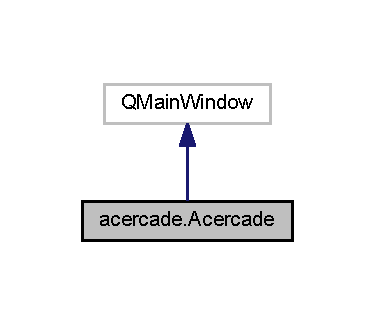
\includegraphics[width=180pt]{classacercade_1_1_acercade__inherit__graph}
\end{center}
\end{figure}


Diagrama de colaboración para acercade.\-Acercade\-:\nopagebreak
\begin{figure}[H]
\begin{center}
\leavevmode
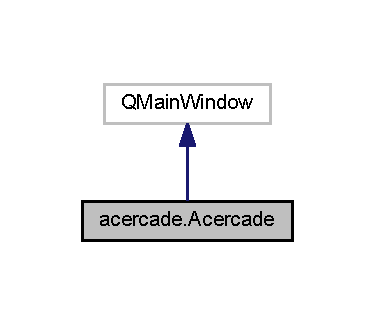
\includegraphics[width=180pt]{classacercade_1_1_acercade__coll__graph}
\end{center}
\end{figure}
\subsection*{Métodos públicos}
\begin{DoxyCompactItemize}
\item 
def {\bf \-\_\-\-\_\-init\-\_\-\-\_\-}
\item 
def {\bf on\-Pushbutton\-Clicked}
\end{DoxyCompactItemize}
\subsection*{Atributos públicos}
\begin{DoxyCompactItemize}
\item 
{\bfseries ui}\label{classacercade_1_1_acercade_a58e39dc112e8ce06be68ba35b2e9df7c}

\item 
{\bfseries p}\label{classacercade_1_1_acercade_a2456e1f5474619d58131f9a5ec5a097f}

\end{DoxyCompactItemize}


\subsection{Descripción detallada}
Clase que corresponde a la ventana acerca de. 

Aqui se mostrara la informacion de los integrantes del grupo desarrollador del juego. 

\subsection{Documentación del constructor y destructor}
\index{acercade\-::\-Acercade@{acercade\-::\-Acercade}!\-\_\-\-\_\-init\-\_\-\-\_\-@{\-\_\-\-\_\-init\-\_\-\-\_\-}}
\index{\-\_\-\-\_\-init\-\_\-\-\_\-@{\-\_\-\-\_\-init\-\_\-\-\_\-}!acercade::Acercade@{acercade\-::\-Acercade}}
\subsubsection[{\-\_\-\-\_\-init\-\_\-\-\_\-}]{\setlength{\rightskip}{0pt plus 5cm}def acercade.\-Acercade.\-\_\-\-\_\-init\-\_\-\-\_\- (
\begin{DoxyParamCaption}
\item[{}]{self}
\end{DoxyParamCaption}
)}\label{classacercade_1_1_acercade_a8552b5cbd085186a1bd2cac854ccc7c3}
\begin{DoxyVerb}Constructor\end{DoxyVerb}
 

\subsection{Documentación de las funciones miembro}
\index{acercade\-::\-Acercade@{acercade\-::\-Acercade}!on\-Pushbutton\-Clicked@{on\-Pushbutton\-Clicked}}
\index{on\-Pushbutton\-Clicked@{on\-Pushbutton\-Clicked}!acercade::Acercade@{acercade\-::\-Acercade}}
\subsubsection[{on\-Pushbutton\-Clicked}]{\setlength{\rightskip}{0pt plus 5cm}def acercade.\-Acercade.\-on\-Pushbutton\-Clicked (
\begin{DoxyParamCaption}
\item[{}]{self}
\end{DoxyParamCaption}
)}\label{classacercade_1_1_acercade_ad6fff0aeaf0378a2d6ba9f0673776933}
\begin{DoxyVerb}maneja evento click boton ok \end{DoxyVerb}
 

La documentación para esta clase fue generada a partir del siguiente fichero\-:\begin{DoxyCompactItemize}
\item 
C\-:/\-Users/\-Kevin/workspace/\-Sudoku\-Python/acercade.\-py\end{DoxyCompactItemize}

\section{Referencia de la Clase graficador.\-Graficador}
\label{classgraficador_1_1_graficador}\index{graficador.\-Graficador@{graficador.\-Graficador}}


clase que se encarga de manejar el color en las fichas en caso de error.  


\subsection*{Métodos públicos}
\begin{DoxyCompactItemize}
\item 
def {\bf \-\_\-\-\_\-init\-\_\-\-\_\-}
\item 
def {\bf init\-Arreglo\-Img\-Fichas}
\item 
def {\bf pinta\-X}
\item 
def {\bf pinta\-Y}
\item 
def {\bf pinta\-Sub}
\item 
def {\bf pinta\-Tablero}
\end{DoxyCompactItemize}
\subsection*{Atributos públicos}
\begin{DoxyCompactItemize}
\item 
{\bfseries sudoku}\label{classgraficador_1_1_graficador_ad833c980c323cc0a8f0c5449b6904410}

\end{DoxyCompactItemize}


\subsection{Descripción detallada}
clase que se encarga de manejar el color en las fichas en caso de error. 

Es utilizada por la clase Sudoku para colorear las fichas cuando existe error en X, en Y, o en la Subcuadricula. 

\subsection{Documentación del constructor y destructor}
\index{graficador\-::\-Graficador@{graficador\-::\-Graficador}!\-\_\-\-\_\-init\-\_\-\-\_\-@{\-\_\-\-\_\-init\-\_\-\-\_\-}}
\index{\-\_\-\-\_\-init\-\_\-\-\_\-@{\-\_\-\-\_\-init\-\_\-\-\_\-}!graficador::Graficador@{graficador\-::\-Graficador}}
\subsubsection[{\-\_\-\-\_\-init\-\_\-\-\_\-}]{\setlength{\rightskip}{0pt plus 5cm}def graficador.\-Graficador.\-\_\-\-\_\-init\-\_\-\-\_\- (
\begin{DoxyParamCaption}
\item[{}]{self, }
\item[{}]{Sudoku}
\end{DoxyParamCaption}
)}\label{classgraficador_1_1_graficador_abf8e67f545b6c08c6e79a86161fe4dea}
\begin{DoxyVerb}Constructor
   parametro:
    s - Nos da la referencia al objeto Sudoku que la crea, para poder acceder a sus variables\end{DoxyVerb}
 

\subsection{Documentación de las funciones miembro}
\index{graficador\-::\-Graficador@{graficador\-::\-Graficador}!init\-Arreglo\-Img\-Fichas@{init\-Arreglo\-Img\-Fichas}}
\index{init\-Arreglo\-Img\-Fichas@{init\-Arreglo\-Img\-Fichas}!graficador::Graficador@{graficador\-::\-Graficador}}
\subsubsection[{init\-Arreglo\-Img\-Fichas}]{\setlength{\rightskip}{0pt plus 5cm}def graficador.\-Graficador.\-init\-Arreglo\-Img\-Fichas (
\begin{DoxyParamCaption}
\item[{}]{self}
\end{DoxyParamCaption}
)}\label{classgraficador_1_1_graficador_aa3d6857907dfdcc6612c474cd9a481f7}
\begin{DoxyVerb}Inicializa un arreglo de Iconos del 1 - 9
    Se asigna a cada elemento del arreglo la imagen de la ficha correspondiente al indice del arreglo.\end{DoxyVerb}
 \index{graficador\-::\-Graficador@{graficador\-::\-Graficador}!pinta\-Sub@{pinta\-Sub}}
\index{pinta\-Sub@{pinta\-Sub}!graficador::Graficador@{graficador\-::\-Graficador}}
\subsubsection[{pinta\-Sub}]{\setlength{\rightskip}{0pt plus 5cm}def graficador.\-Graficador.\-pinta\-Sub (
\begin{DoxyParamCaption}
\item[{}]{self, }
\item[{}]{x, }
\item[{}]{y}
\end{DoxyParamCaption}
)}\label{classgraficador_1_1_graficador_a103831199e9c31836af0698f1ca64483}
\begin{DoxyVerb}Pinta una subcuadricula determinada del tablero cuando hay un error
    Parametro:
x La fila desde donde empieza la subccuadricula en la que se quiere colocar una ficha invalida o incorrecta.
y La columna desde donde empieza la subccuadricula en la que se quiere colocar una ficha invalida o incorrecta\end{DoxyVerb}
 \index{graficador\-::\-Graficador@{graficador\-::\-Graficador}!pinta\-Tablero@{pinta\-Tablero}}
\index{pinta\-Tablero@{pinta\-Tablero}!graficador::Graficador@{graficador\-::\-Graficador}}
\subsubsection[{pinta\-Tablero}]{\setlength{\rightskip}{0pt plus 5cm}def graficador.\-Graficador.\-pinta\-Tablero (
\begin{DoxyParamCaption}
\item[{}]{self}
\end{DoxyParamCaption}
)}\label{classgraficador_1_1_graficador_afb03ec9aafb4068f04ae26d811297edb}
\begin{DoxyVerb}Pinta completamente tablero\end{DoxyVerb}
 \index{graficador\-::\-Graficador@{graficador\-::\-Graficador}!pinta\-X@{pinta\-X}}
\index{pinta\-X@{pinta\-X}!graficador::Graficador@{graficador\-::\-Graficador}}
\subsubsection[{pinta\-X}]{\setlength{\rightskip}{0pt plus 5cm}def graficador.\-Graficador.\-pinta\-X (
\begin{DoxyParamCaption}
\item[{}]{self, }
\item[{}]{i}
\end{DoxyParamCaption}
)}\label{classgraficador_1_1_graficador_a81ed80fb663126b07bb6fc9a20a72d5b}
\begin{DoxyVerb}Pinta una fila determinada del tablero cuando hay un error
   parametro:
   i La fila en la que se quiere colocar una ficha invalida o incorrecta\end{DoxyVerb}
 \index{graficador\-::\-Graficador@{graficador\-::\-Graficador}!pinta\-Y@{pinta\-Y}}
\index{pinta\-Y@{pinta\-Y}!graficador::Graficador@{graficador\-::\-Graficador}}
\subsubsection[{pinta\-Y}]{\setlength{\rightskip}{0pt plus 5cm}def graficador.\-Graficador.\-pinta\-Y (
\begin{DoxyParamCaption}
\item[{}]{self, }
\item[{}]{j}
\end{DoxyParamCaption}
)}\label{classgraficador_1_1_graficador_a7f56a09fa17b5a5aaf7292bff6c2d711}
\begin{DoxyVerb}Pinta una columna determinada del tablero cuando hay un error
   parametro:
       j La columna en la que se quiere colocar una ficha invalida o incorrecta\end{DoxyVerb}
 

La documentación para esta clase fue generada a partir del siguiente fichero\-:\begin{DoxyCompactItemize}
\item 
C\-:/\-Users/\-Kevin/workspace/\-Sudoku\-Python/graficador.\-py\end{DoxyCompactItemize}

\section{Referencia de la Clase nuevojuego.\-Nuevojuego}
\label{classnuevojuego_1_1_nuevojuego}\index{nuevojuego.\-Nuevojuego@{nuevojuego.\-Nuevojuego}}


Clase que corresponde a la ventana de configuracion de opciones para un nuevo juego.  




Diagrama de herencias de nuevojuego.\-Nuevojuego\nopagebreak
\begin{figure}[H]
\begin{center}
\leavevmode
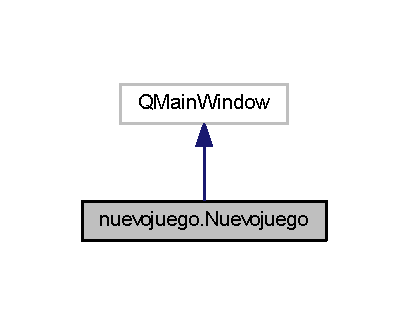
\includegraphics[width=196pt]{classnuevojuego_1_1_nuevojuego__inherit__graph}
\end{center}
\end{figure}


Diagrama de colaboración para nuevojuego.\-Nuevojuego\-:\nopagebreak
\begin{figure}[H]
\begin{center}
\leavevmode
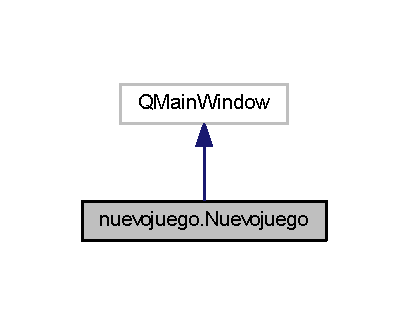
\includegraphics[width=196pt]{classnuevojuego_1_1_nuevojuego__coll__graph}
\end{center}
\end{figure}
\subsection*{Métodos públicos}
\begin{DoxyCompactItemize}
\item 
def {\bf \-\_\-\-\_\-init\-\_\-\-\_\-}
\item 
def {\bf on\-Pbjugar\-Clicked}
\item 
def {\bf on\-Pbcancelar\-Clicked}
\end{DoxyCompactItemize}
\subsection*{Atributos públicos}
\begin{DoxyCompactItemize}
\item 
{\bfseries ui}\label{classnuevojuego_1_1_nuevojuego_adbc8ceb5e6313982e76998d8632c165b}

\item 
{\bfseries Message\-Box}\label{classnuevojuego_1_1_nuevojuego_a0d82932930ca81e673f98e7752fb3401}

\item 
{\bfseries M\-B\-\_\-\-I\-C\-O\-N\-E\-R\-R\-O\-R}\label{classnuevojuego_1_1_nuevojuego_a7dd494e130a721a07a5e4fbf8fbaf26c}

\item 
{\bfseries n}\label{classnuevojuego_1_1_nuevojuego_af9b393a290e8f6a0ffd42a5e0c652549}

\item 
{\bfseries p}\label{classnuevojuego_1_1_nuevojuego_acf09514a8d20e997010bec0eab31105c}

\end{DoxyCompactItemize}


\subsection{Descripción detallada}
Clase que corresponde a la ventana de configuracion de opciones para un nuevo juego. 

Aqui se mostraran 3 secciones\-:

-\/-\/---$>$Dificultad. Se escogen la dificultad deseada.

-\/-\/---$>$Opciones de Alerta. Se escoge que tipos de alerta queremos que nos de la aplicacion al momento de jugar.

-\/-\/---$>$Ayuda. Activamos o desactivamos el boton de ayuda. 

\subsection{Documentación del constructor y destructor}
\index{nuevojuego\-::\-Nuevojuego@{nuevojuego\-::\-Nuevojuego}!\-\_\-\-\_\-init\-\_\-\-\_\-@{\-\_\-\-\_\-init\-\_\-\-\_\-}}
\index{\-\_\-\-\_\-init\-\_\-\-\_\-@{\-\_\-\-\_\-init\-\_\-\-\_\-}!nuevojuego::Nuevojuego@{nuevojuego\-::\-Nuevojuego}}
\subsubsection[{\-\_\-\-\_\-init\-\_\-\-\_\-}]{\setlength{\rightskip}{0pt plus 5cm}def nuevojuego.\-Nuevojuego.\-\_\-\-\_\-init\-\_\-\-\_\- (
\begin{DoxyParamCaption}
\item[{}]{self}
\end{DoxyParamCaption}
)}\label{classnuevojuego_1_1_nuevojuego_aa4e038a99366e2cf8a6a88fdbb863b15}
\begin{DoxyVerb}Contructor
    Setea uno de los dos checkbox de alertas en true y anade el fondo a la ventana.\end{DoxyVerb}
 

\subsection{Documentación de las funciones miembro}
\index{nuevojuego\-::\-Nuevojuego@{nuevojuego\-::\-Nuevojuego}!on\-Pbcancelar\-Clicked@{on\-Pbcancelar\-Clicked}}
\index{on\-Pbcancelar\-Clicked@{on\-Pbcancelar\-Clicked}!nuevojuego::Nuevojuego@{nuevojuego\-::\-Nuevojuego}}
\subsubsection[{on\-Pbcancelar\-Clicked}]{\setlength{\rightskip}{0pt plus 5cm}def nuevojuego.\-Nuevojuego.\-on\-Pbcancelar\-Clicked (
\begin{DoxyParamCaption}
\item[{}]{self}
\end{DoxyParamCaption}
)}\label{classnuevojuego_1_1_nuevojuego_a29dbd3db7a9368c1ec8ea438e1a921d5}
\begin{DoxyVerb}Despliega la ventana anterior
    Crea una instancia de la ventana principal y la muestra\end{DoxyVerb}
 \index{nuevojuego\-::\-Nuevojuego@{nuevojuego\-::\-Nuevojuego}!on\-Pbjugar\-Clicked@{on\-Pbjugar\-Clicked}}
\index{on\-Pbjugar\-Clicked@{on\-Pbjugar\-Clicked}!nuevojuego::Nuevojuego@{nuevojuego\-::\-Nuevojuego}}
\subsubsection[{on\-Pbjugar\-Clicked}]{\setlength{\rightskip}{0pt plus 5cm}def nuevojuego.\-Nuevojuego.\-on\-Pbjugar\-Clicked (
\begin{DoxyParamCaption}
\item[{}]{self}
\end{DoxyParamCaption}
)}\label{classnuevojuego_1_1_nuevojuego_a3dd0f97658c3b305f428260a7d80252d}
\begin{DoxyVerb}Despliega la ventana con el tablero para empezar el juego
    *Crea una instancia de la clase Sudoku y la muestra.
    *Verificara que se halla escogido un solo nivel de dificultad.
    *Verificara que halla escogido al menos una opcion de alerta.\end{DoxyVerb}
 

La documentación para esta clase fue generada a partir del siguiente fichero\-:\begin{DoxyCompactItemize}
\item 
C\-:/\-Users/\-Kevin/workspace/\-Sudoku\-Python/nuevojuego.\-py\end{DoxyCompactItemize}

\section{Referencia de la Clase principal.\-Principal}
\label{classprincipal_1_1_principal}\index{principal.\-Principal@{principal.\-Principal}}


Clase que corresponde a la ventana Inicial.  




Diagrama de herencias de principal.\-Principal\nopagebreak
\begin{figure}[H]
\begin{center}
\leavevmode
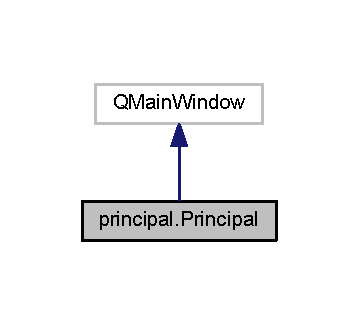
\includegraphics[width=172pt]{classprincipal_1_1_principal__inherit__graph}
\end{center}
\end{figure}


Diagrama de colaboración para principal.\-Principal\-:\nopagebreak
\begin{figure}[H]
\begin{center}
\leavevmode
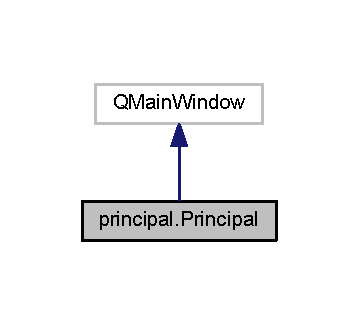
\includegraphics[width=172pt]{classprincipal_1_1_principal__coll__graph}
\end{center}
\end{figure}
\subsection*{Métodos públicos}
\begin{DoxyCompactItemize}
\item 
def {\bf \-\_\-\-\_\-init\-\_\-\-\_\-}
\item 
def {\bf on\-Nuevojuego\-Clicked}
\item 
def {\bf on\-Acercade\-Clicked}
\item 
def {\bf on\-Salir\-Clicked}
\item 
def {\bf on\-Cargajuego\-Clicked}
\end{DoxyCompactItemize}
\subsection*{Atributos públicos}
\begin{DoxyCompactItemize}
\item 
{\bfseries ui}\label{classprincipal_1_1_principal_a93b201004d6c4e4411ae21a7b0ffc555}

\item 
{\bfseries Message\-Box}\label{classprincipal_1_1_principal_a7b6a6c999ee00e401308c673ea04729f}

\item 
{\bfseries M\-B\-\_\-\-I\-C\-O\-N\-E\-R\-R\-O\-R}\label{classprincipal_1_1_principal_a7d119030eaf989c987cc4f4634b489ca}

\item 
{\bfseries n}\label{classprincipal_1_1_principal_a7bb217bc83e234837afcb241611e21e7}

\item 
{\bfseries a}\label{classprincipal_1_1_principal_a75803dbb5436e2218f29d5eb88c0c671}

\end{DoxyCompactItemize}


\subsection{Descripción detallada}
Clase que corresponde a la ventana Inicial. 

Aqui se mostraran 5 diferentes opciones\-:

$\ast$\-Nuevo Juego

$\ast$\-Cargar Juego

$\ast$\-Estadisticas

$\ast$\-Acerca de

$\ast$\-Salir 

\subsection{Documentación del constructor y destructor}
\index{principal\-::\-Principal@{principal\-::\-Principal}!\-\_\-\-\_\-init\-\_\-\-\_\-@{\-\_\-\-\_\-init\-\_\-\-\_\-}}
\index{\-\_\-\-\_\-init\-\_\-\-\_\-@{\-\_\-\-\_\-init\-\_\-\-\_\-}!principal::Principal@{principal\-::\-Principal}}
\subsubsection[{\-\_\-\-\_\-init\-\_\-\-\_\-}]{\setlength{\rightskip}{0pt plus 5cm}def principal.\-Principal.\-\_\-\-\_\-init\-\_\-\-\_\- (
\begin{DoxyParamCaption}
\item[{}]{self}
\end{DoxyParamCaption}
)}\label{classprincipal_1_1_principal_a7f63305aec68ac95f0a9a3dd574e8dc1}
\begin{DoxyVerb}Costructor\end{DoxyVerb}
 

\subsection{Documentación de las funciones miembro}
\index{principal\-::\-Principal@{principal\-::\-Principal}!on\-Acercade\-Clicked@{on\-Acercade\-Clicked}}
\index{on\-Acercade\-Clicked@{on\-Acercade\-Clicked}!principal::Principal@{principal\-::\-Principal}}
\subsubsection[{on\-Acercade\-Clicked}]{\setlength{\rightskip}{0pt plus 5cm}def principal.\-Principal.\-on\-Acercade\-Clicked (
\begin{DoxyParamCaption}
\item[{}]{self}
\end{DoxyParamCaption}
)}\label{classprincipal_1_1_principal_a09645c984cbff6be6ba68c4b95ffbc87}
\begin{DoxyVerb}Muestra informacion del grupo desarrollador\end{DoxyVerb}
 \index{principal\-::\-Principal@{principal\-::\-Principal}!on\-Cargajuego\-Clicked@{on\-Cargajuego\-Clicked}}
\index{on\-Cargajuego\-Clicked@{on\-Cargajuego\-Clicked}!principal::Principal@{principal\-::\-Principal}}
\subsubsection[{on\-Cargajuego\-Clicked}]{\setlength{\rightskip}{0pt plus 5cm}def principal.\-Principal.\-on\-Cargajuego\-Clicked (
\begin{DoxyParamCaption}
\item[{}]{self}
\end{DoxyParamCaption}
)}\label{classprincipal_1_1_principal_a4ba524ec8f9f41be0813a93f52f063a2}
\begin{DoxyVerb}Nos permite Cargar un juego anteriormente guardado\end{DoxyVerb}
 \index{principal\-::\-Principal@{principal\-::\-Principal}!on\-Nuevojuego\-Clicked@{on\-Nuevojuego\-Clicked}}
\index{on\-Nuevojuego\-Clicked@{on\-Nuevojuego\-Clicked}!principal::Principal@{principal\-::\-Principal}}
\subsubsection[{on\-Nuevojuego\-Clicked}]{\setlength{\rightskip}{0pt plus 5cm}def principal.\-Principal.\-on\-Nuevojuego\-Clicked (
\begin{DoxyParamCaption}
\item[{}]{self}
\end{DoxyParamCaption}
)}\label{classprincipal_1_1_principal_ad2d6ac1894d73e687162a5a3541f79e5}
\begin{DoxyVerb}Inicia un nuevo juego
    Crea una instancia de la clase NuevoJuego y la muestra para poder escoger las opciones de juego.\end{DoxyVerb}
 \index{principal\-::\-Principal@{principal\-::\-Principal}!on\-Salir\-Clicked@{on\-Salir\-Clicked}}
\index{on\-Salir\-Clicked@{on\-Salir\-Clicked}!principal::Principal@{principal\-::\-Principal}}
\subsubsection[{on\-Salir\-Clicked}]{\setlength{\rightskip}{0pt plus 5cm}def principal.\-Principal.\-on\-Salir\-Clicked (
\begin{DoxyParamCaption}
\item[{}]{self}
\end{DoxyParamCaption}
)}\label{classprincipal_1_1_principal_a65794ecc2b3264cfb80570925950cfdb}
\begin{DoxyVerb}Nos permite cerrar la aplicacion\end{DoxyVerb}
 

La documentación para esta clase fue generada a partir del siguiente fichero\-:\begin{DoxyCompactItemize}
\item 
C\-:/\-Users/\-Kevin/workspace/\-Sudoku\-Python/principal.\-py\end{DoxyCompactItemize}

\section{Referencia de la Clase sudoku.\-Sudoku}
\label{classsudoku_1_1_sudoku}\index{sudoku.\-Sudoku@{sudoku.\-Sudoku}}


Clase que maneja el tablero.  




Diagrama de herencias de sudoku.\-Sudoku\nopagebreak
\begin{figure}[H]
\begin{center}
\leavevmode
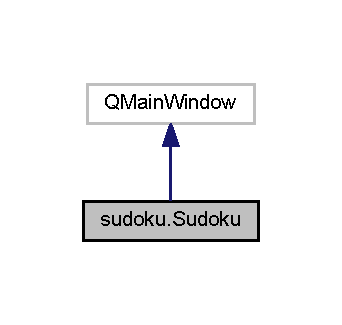
\includegraphics[width=164pt]{classsudoku_1_1_sudoku__inherit__graph}
\end{center}
\end{figure}


Diagrama de colaboración para sudoku.\-Sudoku\-:\nopagebreak
\begin{figure}[H]
\begin{center}
\leavevmode
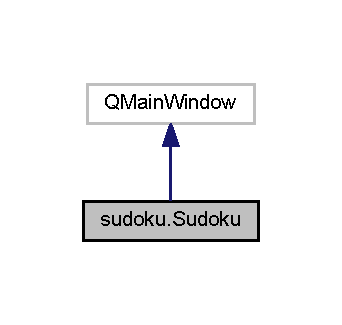
\includegraphics[width=164pt]{classsudoku_1_1_sudoku__coll__graph}
\end{center}
\end{figure}
\subsection*{Métodos públicos}
\begin{DoxyCompactItemize}
\item 
def {\bf \-\_\-\-\_\-init\-\_\-\-\_\-}
\item 
def {\bf init\-Cronometro}
\item 
def {\bf mostrar\-Tiempo}
\item 
def {\bf init\-Gui}
\item 
def {\bf on\-Colocar\-Ficha}
\item 
def {\bf init\-Arreglo\-Pistas}
\item 
def {\bf muestra\-Posibles\-Fichas}
\item 
def {\bf mostrar\-Pistas}
\item 
def {\bf opcion\-Ayuda}
\item 
def {\bf llena\-Tablero\-Dificultad}
\item 
def {\bf set\-Dificultad}
\item 
def {\bf convertir\-Intto\-Img}
\item 
def {\bf jugada\-Incorrecta}
\item 
def {\bf leer\-Archivo\-Sudoku\-Resuelto}
\item 
def {\bf intercambiar\-Filas}
\item 
def {\bf intercambiar\-Columnas}
\item 
def {\bf intercambiar\-Grupo\-Filas}
\item 
def {\bf intercambiar\-Grupo\-Columnas}
\item 
def {\bfseries cargar\-Partida}\label{classsudoku_1_1_sudoku_a686faf15eb72b43e46b639ca832c4f2f}

\item 
def {\bf on\-Pbf1\-Clicked}
\item 
def {\bf on\-Pbf2\-Clicked}
\item 
def {\bf on\-Pbf3\-Clicked}
\item 
def {\bf on\-Pbf4\-Clicked}
\item 
def {\bf on\-Pbf5\-Clicked}
\item 
def {\bf on\-Pbf6\-Clicked}
\item 
def {\bf on\-Pbf7\-Clicked}
\item 
def {\bf on\-Pbf8\-Clicked}
\item 
def {\bf on\-Pbf9\-Clicked}
\item 
def {\bf on\-Bt\-Help\-Clicked}
\item 
def {\bf on\-Actionnuevo\-\_\-juego\-Triggered}
\item 
def {\bf on\-Actionguardar\-Triggered}
\item 
def {\bf on\-Actionsalir\-Triggered}
\end{DoxyCompactItemize}
\subsection*{Atributos públicos}
\begin{DoxyCompactItemize}
\item 
{\bfseries ui}\label{classsudoku_1_1_sudoku_a10cba1664c1eb9e06b1e2be80e491146}

\item 
{\bfseries dificultad}\label{classsudoku_1_1_sudoku_a2967c1d8128e53194947c5663e70318f}

\item 
{\bfseries invalida}\label{classsudoku_1_1_sudoku_aaef20a252919abf513a901c247241a6a}

\item 
{\bfseries incorrecta}\label{classsudoku_1_1_sudoku_a4f4afd0b3785276e719f928474c119dd}

\item 
{\bfseries ayuda}\label{classsudoku_1_1_sudoku_aeb102933d828a4db322986df7ed9c9c5}

\item 
{\bfseries partida}\label{classsudoku_1_1_sudoku_a1280aaf84aa65e77bfcc03d11487e671}

\item 
{\bfseries ayudas}\label{classsudoku_1_1_sudoku_afa5ca87aebb8ea7451b34a357a13d47e}

\item 
{\bfseries validador}\label{classsudoku_1_1_sudoku_a0b10047ea545c0d20858f594ebb33a23}

\item 
{\bfseries Message\-Box}\label{classsudoku_1_1_sudoku_ac82ccedd2ad47903886a0d4d6d0dc72d}

\item 
{\bfseries M\-B\-\_\-\-I\-C\-O\-N\-E\-R\-R\-O\-R}\label{classsudoku_1_1_sudoku_a8b1333d2509e84421b8cd5e13b110895}

\item 
{\bfseries M\-B\-\_\-\-I\-C\-O\-N\-E\-X\-C\-L\-A\-M\-A\-T\-I\-O\-N}\label{classsudoku_1_1_sudoku_a3f05c83e09e7a9ebaa04bf758bc2564d}

\item 
{\bfseries tiempo}\label{classsudoku_1_1_sudoku_af197c9aad28be2bb614b53a7654999a6}

\item 
{\bfseries timer}\label{classsudoku_1_1_sudoku_a0da495ba22f336a9d6593d80be5e8a8a}

\item 
{\bfseries segundos}\label{classsudoku_1_1_sudoku_a681d3ae6b17d362ee8e4e0b0985fe6b6}

\item 
{\bfseries text}\label{classsudoku_1_1_sudoku_a3ef9b3cb73521c03fc13a55195371df6}

\item 
{\bfseries nuevo\-Tiempo}\label{classsudoku_1_1_sudoku_ab54f34d9121b3d949b15e26053121a60}

\item 
{\bfseries cronometro}\label{classsudoku_1_1_sudoku_aecc1384833d05b2f20df9ed4b085965c}

\item 
{\bfseries Bmetodo}\label{classsudoku_1_1_sudoku_abd8e43ea44fb20adb86165a0b36a1dcc}

\item 
{\bfseries cajas}\label{classsudoku_1_1_sudoku_ae70a9aa78c648f9bb01457db5e9ad14e}

\item 
{\bfseries numero}\label{classsudoku_1_1_sudoku_ad01be06931dc273aa73327c23923ddac}

\item 
{\bfseries pos\-Fichas}\label{classsudoku_1_1_sudoku_ae29c470920cd2318f8103d209e278a9f}

\item 
{\bfseries nro\-Fichas}\label{classsudoku_1_1_sudoku_ace939fd0f2355c195b77d66a256cd6e7}

\item 
{\bfseries resuelto}\label{classsudoku_1_1_sudoku_a8eb9dd56067013c106d40d66d16dbc54}

\item 
{\bfseries n}\label{classsudoku_1_1_sudoku_a622ecbe2563df85e66af316d2c075388}

\end{DoxyCompactItemize}


\subsection{Descripción detallada}
Clase que maneja el tablero. 

Aqui se genera el tablero de acuerdo con las especificaciones dadas desde la ventana de nuevo juego como las opciones de alerta, la dificultad y la ayuda. 

\subsection{Documentación del constructor y destructor}
\index{sudoku\-::\-Sudoku@{sudoku\-::\-Sudoku}!\-\_\-\-\_\-init\-\_\-\-\_\-@{\-\_\-\-\_\-init\-\_\-\-\_\-}}
\index{\-\_\-\-\_\-init\-\_\-\-\_\-@{\-\_\-\-\_\-init\-\_\-\-\_\-}!sudoku::Sudoku@{sudoku\-::\-Sudoku}}
\subsubsection[{\-\_\-\-\_\-init\-\_\-\-\_\-}]{\setlength{\rightskip}{0pt plus 5cm}def sudoku.\-Sudoku.\-\_\-\-\_\-init\-\_\-\-\_\- (
\begin{DoxyParamCaption}
\item[{}]{self, }
\item[{}]{dificultad, }
\item[{}]{invalida, }
\item[{}]{incorrecta, }
\item[{}]{ayuda, }
\item[{}]{partida}
\end{DoxyParamCaption}
)}\label{classsudoku_1_1_sudoku_a14eb9b8b5458e35cbed1faf30e761294}
\begin{DoxyVerb}Contructor
    *Crea una instancia de Sudoku de acuerdo a las especificaciones dadas por las variables de entrada.
    *Se crea e inicia el cronometro.
    Parametro:
    - dificultad Dificultad del juego.
    - incorrecta Determina si se realizan o no las validaciones de jugadas incorrectas.
    - invalida Determina si se realizan o no las validaciones de jugadas invalidas.
    - ayuda Determina si se activa o no el boton ayuda.\end{DoxyVerb}
 

\subsection{Documentación de las funciones miembro}
\index{sudoku\-::\-Sudoku@{sudoku\-::\-Sudoku}!convertir\-Intto\-Img@{convertir\-Intto\-Img}}
\index{convertir\-Intto\-Img@{convertir\-Intto\-Img}!sudoku::Sudoku@{sudoku\-::\-Sudoku}}
\subsubsection[{convertir\-Intto\-Img}]{\setlength{\rightskip}{0pt plus 5cm}def sudoku.\-Sudoku.\-convertir\-Intto\-Img (
\begin{DoxyParamCaption}
\item[{}]{self}
\end{DoxyParamCaption}
)}\label{classsudoku_1_1_sudoku_abf1e37a0ceed64e3c928ec5f1b029aa2}
\begin{DoxyVerb}Convierte el numero que se encuentra el la matriz Modelo a una ficha.\end{DoxyVerb}
 \index{sudoku\-::\-Sudoku@{sudoku\-::\-Sudoku}!init\-Arreglo\-Pistas@{init\-Arreglo\-Pistas}}
\index{init\-Arreglo\-Pistas@{init\-Arreglo\-Pistas}!sudoku::Sudoku@{sudoku\-::\-Sudoku}}
\subsubsection[{init\-Arreglo\-Pistas}]{\setlength{\rightskip}{0pt plus 5cm}def sudoku.\-Sudoku.\-init\-Arreglo\-Pistas (
\begin{DoxyParamCaption}
\item[{}]{self}
\end{DoxyParamCaption}
)}\label{classsudoku_1_1_sudoku_af983841e936a54c492cd19d1894fbd62}
\begin{DoxyVerb}Inicializa el arreglo al principio con fichas vacias\end{DoxyVerb}
 \index{sudoku\-::\-Sudoku@{sudoku\-::\-Sudoku}!init\-Cronometro@{init\-Cronometro}}
\index{init\-Cronometro@{init\-Cronometro}!sudoku::Sudoku@{sudoku\-::\-Sudoku}}
\subsubsection[{init\-Cronometro}]{\setlength{\rightskip}{0pt plus 5cm}def sudoku.\-Sudoku.\-init\-Cronometro (
\begin{DoxyParamCaption}
\item[{}]{self}
\end{DoxyParamCaption}
)}\label{classsudoku_1_1_sudoku_a3614de81f1066c542488693a403432da}
\begin{DoxyVerb}Inicia el contador del cronometro\end{DoxyVerb}
 \index{sudoku\-::\-Sudoku@{sudoku\-::\-Sudoku}!init\-Gui@{init\-Gui}}
\index{init\-Gui@{init\-Gui}!sudoku::Sudoku@{sudoku\-::\-Sudoku}}
\subsubsection[{init\-Gui}]{\setlength{\rightskip}{0pt plus 5cm}def sudoku.\-Sudoku.\-init\-Gui (
\begin{DoxyParamCaption}
\item[{}]{self}
\end{DoxyParamCaption}
)}\label{classsudoku_1_1_sudoku_ac33d986fc4b8d7f117a335a1cf972425}
\begin{DoxyVerb}Inicializa la interfaz grafica del tablero
    Se inicializa el tablero y luego se lo llena con el numero de fichas de acuerdo a la dificultad.\end{DoxyVerb}
 \index{sudoku\-::\-Sudoku@{sudoku\-::\-Sudoku}!intercambiar\-Columnas@{intercambiar\-Columnas}}
\index{intercambiar\-Columnas@{intercambiar\-Columnas}!sudoku::Sudoku@{sudoku\-::\-Sudoku}}
\subsubsection[{intercambiar\-Columnas}]{\setlength{\rightskip}{0pt plus 5cm}def sudoku.\-Sudoku.\-intercambiar\-Columnas (
\begin{DoxyParamCaption}
\item[{}]{self}
\end{DoxyParamCaption}
)}\label{classsudoku_1_1_sudoku_ac1bfe63c57091eba26b0a7798ebf651c}
\begin{DoxyVerb}Realiza un intercambio aleatorio de las columnas dentro de las subcuadriculas\end{DoxyVerb}
 \index{sudoku\-::\-Sudoku@{sudoku\-::\-Sudoku}!intercambiar\-Filas@{intercambiar\-Filas}}
\index{intercambiar\-Filas@{intercambiar\-Filas}!sudoku::Sudoku@{sudoku\-::\-Sudoku}}
\subsubsection[{intercambiar\-Filas}]{\setlength{\rightskip}{0pt plus 5cm}def sudoku.\-Sudoku.\-intercambiar\-Filas (
\begin{DoxyParamCaption}
\item[{}]{self}
\end{DoxyParamCaption}
)}\label{classsudoku_1_1_sudoku_ac0f0071bbf7e20b46db0922853e4f18c}
\begin{DoxyVerb}Realiza un intercambio aleatorio de las filas dentro de las subcuadriculas\end{DoxyVerb}
 \index{sudoku\-::\-Sudoku@{sudoku\-::\-Sudoku}!intercambiar\-Grupo\-Columnas@{intercambiar\-Grupo\-Columnas}}
\index{intercambiar\-Grupo\-Columnas@{intercambiar\-Grupo\-Columnas}!sudoku::Sudoku@{sudoku\-::\-Sudoku}}
\subsubsection[{intercambiar\-Grupo\-Columnas}]{\setlength{\rightskip}{0pt plus 5cm}def sudoku.\-Sudoku.\-intercambiar\-Grupo\-Columnas (
\begin{DoxyParamCaption}
\item[{}]{self}
\end{DoxyParamCaption}
)}\label{classsudoku_1_1_sudoku_a88a5f6c4d65c50bce704e9baf37e9a6c}
\begin{DoxyVerb}Realiza un intercambio aleatorio de columnas de subcuadriculas dentro del tablero\end{DoxyVerb}
 \index{sudoku\-::\-Sudoku@{sudoku\-::\-Sudoku}!intercambiar\-Grupo\-Filas@{intercambiar\-Grupo\-Filas}}
\index{intercambiar\-Grupo\-Filas@{intercambiar\-Grupo\-Filas}!sudoku::Sudoku@{sudoku\-::\-Sudoku}}
\subsubsection[{intercambiar\-Grupo\-Filas}]{\setlength{\rightskip}{0pt plus 5cm}def sudoku.\-Sudoku.\-intercambiar\-Grupo\-Filas (
\begin{DoxyParamCaption}
\item[{}]{self}
\end{DoxyParamCaption}
)}\label{classsudoku_1_1_sudoku_a056c8e4f7ca6d7a6e3ed65aac8c455c8}
\begin{DoxyVerb}Realiza un intercambio aleatorio de filas de subcuadriculas dentro del tablero\end{DoxyVerb}
 \index{sudoku\-::\-Sudoku@{sudoku\-::\-Sudoku}!jugada\-Incorrecta@{jugada\-Incorrecta}}
\index{jugada\-Incorrecta@{jugada\-Incorrecta}!sudoku::Sudoku@{sudoku\-::\-Sudoku}}
\subsubsection[{jugada\-Incorrecta}]{\setlength{\rightskip}{0pt plus 5cm}def sudoku.\-Sudoku.\-jugada\-Incorrecta (
\begin{DoxyParamCaption}
\item[{}]{self, }
\item[{}]{indice}
\end{DoxyParamCaption}
)}\label{classsudoku_1_1_sudoku_a56bd70c70ad08e350a33f9eafd5747d5}
\begin{DoxyVerb}Determina si la jugada es Incorrecta
    *Compara el numero que el jugador desea colocar con el numero que esta en esa misma posicion del tablero solucionado.
    Parametro: ind El indice del boton correspondiente al lugar donde el jugador desea colocar la ficha.
    Retorna: 1 -> Incorrecto , 0 -> Correcto.\end{DoxyVerb}
 \index{sudoku\-::\-Sudoku@{sudoku\-::\-Sudoku}!leer\-Archivo\-Sudoku\-Resuelto@{leer\-Archivo\-Sudoku\-Resuelto}}
\index{leer\-Archivo\-Sudoku\-Resuelto@{leer\-Archivo\-Sudoku\-Resuelto}!sudoku::Sudoku@{sudoku\-::\-Sudoku}}
\subsubsection[{leer\-Archivo\-Sudoku\-Resuelto}]{\setlength{\rightskip}{0pt plus 5cm}def sudoku.\-Sudoku.\-leer\-Archivo\-Sudoku\-Resuelto (
\begin{DoxyParamCaption}
\item[{}]{self}
\end{DoxyParamCaption}
)}\label{classsudoku_1_1_sudoku_a199b4fbc1f49e61904a084c2a11d6ca7}
\begin{DoxyVerb}Lee el archivo de texto encriptado y llena el arreglo con el sudoku resuelto\end{DoxyVerb}
 \index{sudoku\-::\-Sudoku@{sudoku\-::\-Sudoku}!llena\-Tablero\-Dificultad@{llena\-Tablero\-Dificultad}}
\index{llena\-Tablero\-Dificultad@{llena\-Tablero\-Dificultad}!sudoku::Sudoku@{sudoku\-::\-Sudoku}}
\subsubsection[{llena\-Tablero\-Dificultad}]{\setlength{\rightskip}{0pt plus 5cm}def sudoku.\-Sudoku.\-llena\-Tablero\-Dificultad (
\begin{DoxyParamCaption}
\item[{}]{self}
\end{DoxyParamCaption}
)}\label{classsudoku_1_1_sudoku_acbda245010d2545e9b37c7c1769e709f}
\begin{DoxyVerb}Llena el tablero que se mostrara al jugador de acuerdo a la dificultad que se eligio
    Se asigna el numero de fichas de acuerdo con la dificultad en posiciones aleatorias.\end{DoxyVerb}
 \index{sudoku\-::\-Sudoku@{sudoku\-::\-Sudoku}!mostrar\-Pistas@{mostrar\-Pistas}}
\index{mostrar\-Pistas@{mostrar\-Pistas}!sudoku::Sudoku@{sudoku\-::\-Sudoku}}
\subsubsection[{mostrar\-Pistas}]{\setlength{\rightskip}{0pt plus 5cm}def sudoku.\-Sudoku.\-mostrar\-Pistas (
\begin{DoxyParamCaption}
\item[{}]{self}
\end{DoxyParamCaption}
)}\label{classsudoku_1_1_sudoku_ad8cceb57016ac37ab305c54287876745}
\begin{DoxyVerb}Agrega las posibles fichas en la ventana\end{DoxyVerb}
 \index{sudoku\-::\-Sudoku@{sudoku\-::\-Sudoku}!mostrar\-Tiempo@{mostrar\-Tiempo}}
\index{mostrar\-Tiempo@{mostrar\-Tiempo}!sudoku::Sudoku@{sudoku\-::\-Sudoku}}
\subsubsection[{mostrar\-Tiempo}]{\setlength{\rightskip}{0pt plus 5cm}def sudoku.\-Sudoku.\-mostrar\-Tiempo (
\begin{DoxyParamCaption}
\item[{}]{self}
\end{DoxyParamCaption}
)}\label{classsudoku_1_1_sudoku_a79a4ebb6cba45ec5aa3464c70f12535a}
\begin{DoxyVerb}Controla el aumento de los segundos\end{DoxyVerb}
 \index{sudoku\-::\-Sudoku@{sudoku\-::\-Sudoku}!muestra\-Posibles\-Fichas@{muestra\-Posibles\-Fichas}}
\index{muestra\-Posibles\-Fichas@{muestra\-Posibles\-Fichas}!sudoku::Sudoku@{sudoku\-::\-Sudoku}}
\subsubsection[{muestra\-Posibles\-Fichas}]{\setlength{\rightskip}{0pt plus 5cm}def sudoku.\-Sudoku.\-muestra\-Posibles\-Fichas (
\begin{DoxyParamCaption}
\item[{}]{self, }
\item[{}]{caja}
\end{DoxyParamCaption}
)}\label{classsudoku_1_1_sudoku_af086075fea0c4691e901ccb64b92f0d2}
\begin{DoxyVerb}Muestra las fichas que son validas para esa posicion.
    Parametro: button Boton en la posicion donde se desea colocar la ficha.\end{DoxyVerb}
 \index{sudoku\-::\-Sudoku@{sudoku\-::\-Sudoku}!on\-Actionguardar\-Triggered@{on\-Actionguardar\-Triggered}}
\index{on\-Actionguardar\-Triggered@{on\-Actionguardar\-Triggered}!sudoku::Sudoku@{sudoku\-::\-Sudoku}}
\subsubsection[{on\-Actionguardar\-Triggered}]{\setlength{\rightskip}{0pt plus 5cm}def sudoku.\-Sudoku.\-on\-Actionguardar\-Triggered (
\begin{DoxyParamCaption}
\item[{}]{self}
\end{DoxyParamCaption}
)}\label{classsudoku_1_1_sudoku_a04e410b502daf2b7dba261c7c1890fa8}
\begin{DoxyVerb}Guarda la partida actual
    Se pide el nombre con el que se desea guardar la partida y luego se procede a grabarla con encriptacion.\end{DoxyVerb}
 \index{sudoku\-::\-Sudoku@{sudoku\-::\-Sudoku}!on\-Actionnuevo\-\_\-juego\-Triggered@{on\-Actionnuevo\-\_\-juego\-Triggered}}
\index{on\-Actionnuevo\-\_\-juego\-Triggered@{on\-Actionnuevo\-\_\-juego\-Triggered}!sudoku::Sudoku@{sudoku\-::\-Sudoku}}
\subsubsection[{on\-Actionnuevo\-\_\-juego\-Triggered}]{\setlength{\rightskip}{0pt plus 5cm}def sudoku.\-Sudoku.\-on\-Actionnuevo\-\_\-juego\-Triggered (
\begin{DoxyParamCaption}
\item[{}]{self}
\end{DoxyParamCaption}
)}\label{classsudoku_1_1_sudoku_a9d461c3559ed288877a00055da014eba}
\begin{DoxyVerb}Despliega la ventana de nuevo juego\end{DoxyVerb}
 \index{sudoku\-::\-Sudoku@{sudoku\-::\-Sudoku}!on\-Actionsalir\-Triggered@{on\-Actionsalir\-Triggered}}
\index{on\-Actionsalir\-Triggered@{on\-Actionsalir\-Triggered}!sudoku::Sudoku@{sudoku\-::\-Sudoku}}
\subsubsection[{on\-Actionsalir\-Triggered}]{\setlength{\rightskip}{0pt plus 5cm}def sudoku.\-Sudoku.\-on\-Actionsalir\-Triggered (
\begin{DoxyParamCaption}
\item[{}]{self}
\end{DoxyParamCaption}
)}\label{classsudoku_1_1_sudoku_aa96e09f95d70580e45a0af6e23e4ab64}
\begin{DoxyVerb}Salir de la partida actual.\end{DoxyVerb}
 \index{sudoku\-::\-Sudoku@{sudoku\-::\-Sudoku}!on\-Bt\-Help\-Clicked@{on\-Bt\-Help\-Clicked}}
\index{on\-Bt\-Help\-Clicked@{on\-Bt\-Help\-Clicked}!sudoku::Sudoku@{sudoku\-::\-Sudoku}}
\subsubsection[{on\-Bt\-Help\-Clicked}]{\setlength{\rightskip}{0pt plus 5cm}def sudoku.\-Sudoku.\-on\-Bt\-Help\-Clicked (
\begin{DoxyParamCaption}
\item[{}]{self}
\end{DoxyParamCaption}
)}\label{classsudoku_1_1_sudoku_a18055f16332f25d54471b01ad7a4283b}
\begin{DoxyVerb}Setea el numero 0 que indicara que se va a colocar el numero correcto automaticamente.\end{DoxyVerb}
 \index{sudoku\-::\-Sudoku@{sudoku\-::\-Sudoku}!on\-Colocar\-Ficha@{on\-Colocar\-Ficha}}
\index{on\-Colocar\-Ficha@{on\-Colocar\-Ficha}!sudoku::Sudoku@{sudoku\-::\-Sudoku}}
\subsubsection[{on\-Colocar\-Ficha}]{\setlength{\rightskip}{0pt plus 5cm}def sudoku.\-Sudoku.\-on\-Colocar\-Ficha (
\begin{DoxyParamCaption}
\item[{}]{self}
\end{DoxyParamCaption}
)}\label{classsudoku_1_1_sudoku_ab90f4256f9ca764774df6c606dccb8bc}
\begin{DoxyVerb}Slot que se ejecuta cada vez que se presione en algun boton dentro del tablero
 Determina que accion se realiza al pulsar la ficha en el tablero.
 Controla que tipo de validacion se realiza.\end{DoxyVerb}
 \index{sudoku\-::\-Sudoku@{sudoku\-::\-Sudoku}!on\-Pbf1\-Clicked@{on\-Pbf1\-Clicked}}
\index{on\-Pbf1\-Clicked@{on\-Pbf1\-Clicked}!sudoku::Sudoku@{sudoku\-::\-Sudoku}}
\subsubsection[{on\-Pbf1\-Clicked}]{\setlength{\rightskip}{0pt plus 5cm}def sudoku.\-Sudoku.\-on\-Pbf1\-Clicked (
\begin{DoxyParamCaption}
\item[{}]{self}
\end{DoxyParamCaption}
)}\label{classsudoku_1_1_sudoku_af636ad3dd5ecf0586b5a0cc11bbc0e78}
\begin{DoxyVerb}Setea el numero 1 siendo esta ficha la que el jugador quiere colocar en alguna parte del tablero.\end{DoxyVerb}
 \index{sudoku\-::\-Sudoku@{sudoku\-::\-Sudoku}!on\-Pbf2\-Clicked@{on\-Pbf2\-Clicked}}
\index{on\-Pbf2\-Clicked@{on\-Pbf2\-Clicked}!sudoku::Sudoku@{sudoku\-::\-Sudoku}}
\subsubsection[{on\-Pbf2\-Clicked}]{\setlength{\rightskip}{0pt plus 5cm}def sudoku.\-Sudoku.\-on\-Pbf2\-Clicked (
\begin{DoxyParamCaption}
\item[{}]{self}
\end{DoxyParamCaption}
)}\label{classsudoku_1_1_sudoku_a2da5196b891674fe7d9e4f1c12b8f3d4}
\begin{DoxyVerb}Setea el numero 2 siendo esta ficha la que el jugador quiere colocar en alguna parte del tablero.\end{DoxyVerb}
 \index{sudoku\-::\-Sudoku@{sudoku\-::\-Sudoku}!on\-Pbf3\-Clicked@{on\-Pbf3\-Clicked}}
\index{on\-Pbf3\-Clicked@{on\-Pbf3\-Clicked}!sudoku::Sudoku@{sudoku\-::\-Sudoku}}
\subsubsection[{on\-Pbf3\-Clicked}]{\setlength{\rightskip}{0pt plus 5cm}def sudoku.\-Sudoku.\-on\-Pbf3\-Clicked (
\begin{DoxyParamCaption}
\item[{}]{self}
\end{DoxyParamCaption}
)}\label{classsudoku_1_1_sudoku_a36c26f1d64db573765430a916a4b845a}
\begin{DoxyVerb}Setea el numero 3 siendo esta ficha la que el jugador quiere colocar en alguna parte del tablero.\end{DoxyVerb}
 \index{sudoku\-::\-Sudoku@{sudoku\-::\-Sudoku}!on\-Pbf4\-Clicked@{on\-Pbf4\-Clicked}}
\index{on\-Pbf4\-Clicked@{on\-Pbf4\-Clicked}!sudoku::Sudoku@{sudoku\-::\-Sudoku}}
\subsubsection[{on\-Pbf4\-Clicked}]{\setlength{\rightskip}{0pt plus 5cm}def sudoku.\-Sudoku.\-on\-Pbf4\-Clicked (
\begin{DoxyParamCaption}
\item[{}]{self}
\end{DoxyParamCaption}
)}\label{classsudoku_1_1_sudoku_a6f13726fd8cad20874d2f66c93fb6a7a}
\begin{DoxyVerb}Setea el numero 4 siendo esta ficha la que el jugador quiere colocar en alguna parte del tablero.\end{DoxyVerb}
 \index{sudoku\-::\-Sudoku@{sudoku\-::\-Sudoku}!on\-Pbf5\-Clicked@{on\-Pbf5\-Clicked}}
\index{on\-Pbf5\-Clicked@{on\-Pbf5\-Clicked}!sudoku::Sudoku@{sudoku\-::\-Sudoku}}
\subsubsection[{on\-Pbf5\-Clicked}]{\setlength{\rightskip}{0pt plus 5cm}def sudoku.\-Sudoku.\-on\-Pbf5\-Clicked (
\begin{DoxyParamCaption}
\item[{}]{self}
\end{DoxyParamCaption}
)}\label{classsudoku_1_1_sudoku_a0e6b40f43c2846d6895866461df4904a}
\begin{DoxyVerb}Setea el numero 5 siendo esta ficha la que el jugador quiere colocar en alguna parte del tablero.\end{DoxyVerb}
 \index{sudoku\-::\-Sudoku@{sudoku\-::\-Sudoku}!on\-Pbf6\-Clicked@{on\-Pbf6\-Clicked}}
\index{on\-Pbf6\-Clicked@{on\-Pbf6\-Clicked}!sudoku::Sudoku@{sudoku\-::\-Sudoku}}
\subsubsection[{on\-Pbf6\-Clicked}]{\setlength{\rightskip}{0pt plus 5cm}def sudoku.\-Sudoku.\-on\-Pbf6\-Clicked (
\begin{DoxyParamCaption}
\item[{}]{self}
\end{DoxyParamCaption}
)}\label{classsudoku_1_1_sudoku_abb607fa3fc51befda78e7425b7200ddd}
\begin{DoxyVerb}Setea el numero 6 siendo esta ficha la que el jugador quiere colocar en alguna parte del tablero.\end{DoxyVerb}
 \index{sudoku\-::\-Sudoku@{sudoku\-::\-Sudoku}!on\-Pbf7\-Clicked@{on\-Pbf7\-Clicked}}
\index{on\-Pbf7\-Clicked@{on\-Pbf7\-Clicked}!sudoku::Sudoku@{sudoku\-::\-Sudoku}}
\subsubsection[{on\-Pbf7\-Clicked}]{\setlength{\rightskip}{0pt plus 5cm}def sudoku.\-Sudoku.\-on\-Pbf7\-Clicked (
\begin{DoxyParamCaption}
\item[{}]{self}
\end{DoxyParamCaption}
)}\label{classsudoku_1_1_sudoku_af42f0ecb5c36080dbe2a03d00e92c0aa}
\begin{DoxyVerb}Setea el numero 7 siendo esta ficha la que el jugador quiere colocar en alguna parte del tablero.\end{DoxyVerb}
 \index{sudoku\-::\-Sudoku@{sudoku\-::\-Sudoku}!on\-Pbf8\-Clicked@{on\-Pbf8\-Clicked}}
\index{on\-Pbf8\-Clicked@{on\-Pbf8\-Clicked}!sudoku::Sudoku@{sudoku\-::\-Sudoku}}
\subsubsection[{on\-Pbf8\-Clicked}]{\setlength{\rightskip}{0pt plus 5cm}def sudoku.\-Sudoku.\-on\-Pbf8\-Clicked (
\begin{DoxyParamCaption}
\item[{}]{self}
\end{DoxyParamCaption}
)}\label{classsudoku_1_1_sudoku_a85eed190edf1bbfe3cb4908bb71377ee}
\begin{DoxyVerb}Setea el numero 8 siendo esta ficha la que el jugador quiere colocar en alguna parte del tablero.\end{DoxyVerb}
 \index{sudoku\-::\-Sudoku@{sudoku\-::\-Sudoku}!on\-Pbf9\-Clicked@{on\-Pbf9\-Clicked}}
\index{on\-Pbf9\-Clicked@{on\-Pbf9\-Clicked}!sudoku::Sudoku@{sudoku\-::\-Sudoku}}
\subsubsection[{on\-Pbf9\-Clicked}]{\setlength{\rightskip}{0pt plus 5cm}def sudoku.\-Sudoku.\-on\-Pbf9\-Clicked (
\begin{DoxyParamCaption}
\item[{}]{self}
\end{DoxyParamCaption}
)}\label{classsudoku_1_1_sudoku_a86fc5361d5e951a1b4ee39d9b0203a02}
\begin{DoxyVerb}Setea el numero 9 siendo esta ficha la que el jugador quiere colocar en alguna parte del tablero.\end{DoxyVerb}
 \index{sudoku\-::\-Sudoku@{sudoku\-::\-Sudoku}!opcion\-Ayuda@{opcion\-Ayuda}}
\index{opcion\-Ayuda@{opcion\-Ayuda}!sudoku::Sudoku@{sudoku\-::\-Sudoku}}
\subsubsection[{opcion\-Ayuda}]{\setlength{\rightskip}{0pt plus 5cm}def sudoku.\-Sudoku.\-opcion\-Ayuda (
\begin{DoxyParamCaption}
\item[{}]{self, }
\item[{}]{caja}
\end{DoxyParamCaption}
)}\label{classsudoku_1_1_sudoku_ab5193226c263210588b833b0a24e5cdf}
\begin{DoxyVerb}Maneja la opcion cuando el jugador activa la ayuda
    Parametro: b El boton que corresponde al lugar del tablero donde el jugador desea se coloque el numero correcto.\end{DoxyVerb}
 \index{sudoku\-::\-Sudoku@{sudoku\-::\-Sudoku}!set\-Dificultad@{set\-Dificultad}}
\index{set\-Dificultad@{set\-Dificultad}!sudoku::Sudoku@{sudoku\-::\-Sudoku}}
\subsubsection[{set\-Dificultad}]{\setlength{\rightskip}{0pt plus 5cm}def sudoku.\-Sudoku.\-set\-Dificultad (
\begin{DoxyParamCaption}
\item[{}]{self}
\end{DoxyParamCaption}
)}\label{classsudoku_1_1_sudoku_a291d09df1082915d723befb440762013}
\begin{DoxyVerb}Lee la dificultad y se asigna el numero de fichas correspondiente a dicha dificultad.\end{DoxyVerb}
 

La documentación para esta clase fue generada a partir del siguiente fichero\-:\begin{DoxyCompactItemize}
\item 
C\-:/\-Users/\-Kevin/workspace/\-Sudoku\-Python/sudoku.\-py\end{DoxyCompactItemize}

\section{Referencia de la Clase ui\-\_\-acercade.\-Ui\-\_\-acerca\-De}
\label{classui__acercade_1_1_ui__acerca_de}\index{ui\-\_\-acercade.\-Ui\-\_\-acerca\-De@{ui\-\_\-acercade.\-Ui\-\_\-acerca\-De}}


Diagrama de herencias de ui\-\_\-acercade.\-Ui\-\_\-acerca\-De\nopagebreak
\begin{figure}[H]
\begin{center}
\leavevmode
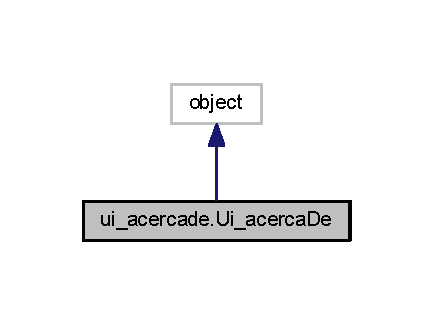
\includegraphics[width=208pt]{classui__acercade_1_1_ui__acerca_de__inherit__graph}
\end{center}
\end{figure}


Diagrama de colaboración para ui\-\_\-acercade.\-Ui\-\_\-acerca\-De\-:\nopagebreak
\begin{figure}[H]
\begin{center}
\leavevmode
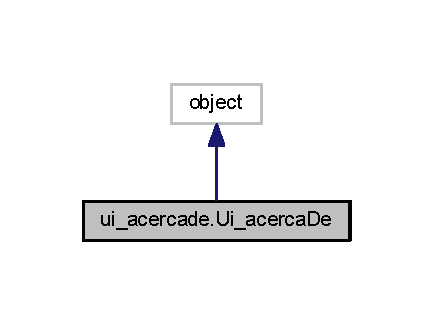
\includegraphics[width=208pt]{classui__acercade_1_1_ui__acerca_de__coll__graph}
\end{center}
\end{figure}
\subsection*{Métodos públicos}
\begin{DoxyCompactItemize}
\item 
def {\bfseries setup\-Ui}\label{classui__acercade_1_1_ui__acerca_de_a2fce16d29c65ead27ca1123784d6ee8c}

\item 
def {\bfseries retranslate\-Ui}\label{classui__acercade_1_1_ui__acerca_de_af7f3107643db084e29df61257d791125}

\end{DoxyCompactItemize}
\subsection*{Atributos públicos}
\begin{DoxyCompactItemize}
\item 
{\bfseries centralwidget}\label{classui__acercade_1_1_ui__acerca_de_a95e78d45d17d029878bda51d82f560bd}

\item 
{\bfseries label}\label{classui__acercade_1_1_ui__acerca_de_add63f6385b5cf6cdc30660422bff4f4e}

\item 
{\bfseries label\-\_\-2}\label{classui__acercade_1_1_ui__acerca_de_af5b713d3263b9ce93ac34a62f1fa8335}

\item 
{\bfseries label\-\_\-3}\label{classui__acercade_1_1_ui__acerca_de_acc09e03251d385b6847e826e00212deb}

\item 
{\bfseries label\-\_\-4}\label{classui__acercade_1_1_ui__acerca_de_ad601633dd874fef63408f5f516b0126b}

\item 
{\bfseries label\-\_\-5}\label{classui__acercade_1_1_ui__acerca_de_aba0f1a1d551e469db2ca5ea1ed88c79a}

\item 
{\bfseries label\-\_\-6}\label{classui__acercade_1_1_ui__acerca_de_aaae4e9fa8e2c464f02108ce9597fc23e}

\item 
{\bfseries push\-Button}\label{classui__acercade_1_1_ui__acerca_de_a3cf0beb8bb91aa01a42525db4f3d89ec}

\end{DoxyCompactItemize}


La documentación para esta clase fue generada a partir del siguiente fichero\-:\begin{DoxyCompactItemize}
\item 
C\-:/\-Users/\-Kevin/workspace/\-Sudoku\-Python/ui\-\_\-acercade.\-py\end{DoxyCompactItemize}

\section{Referencia de la Clase ui\-\_\-estadisticas.\-Ui\-\_\-estadisticas}
\label{classui__estadisticas_1_1_ui__estadisticas}\index{ui\-\_\-estadisticas.\-Ui\-\_\-estadisticas@{ui\-\_\-estadisticas.\-Ui\-\_\-estadisticas}}


Diagrama de herencias de ui\-\_\-estadisticas.\-Ui\-\_\-estadisticas
\nopagebreak
\begin{figure}[H]
\begin{center}
\leavevmode
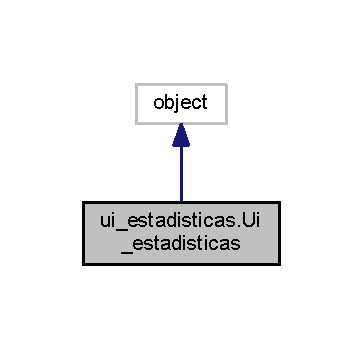
\includegraphics[width=174pt]{classui__estadisticas_1_1_ui__estadisticas__inherit__graph}
\end{center}
\end{figure}


Diagrama de colaboración para ui\-\_\-estadisticas.\-Ui\-\_\-estadisticas\-:
\nopagebreak
\begin{figure}[H]
\begin{center}
\leavevmode
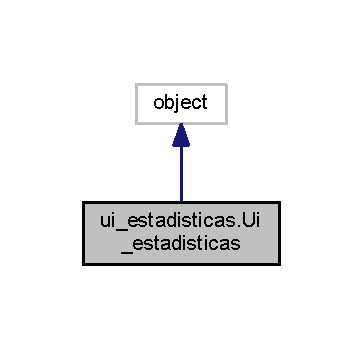
\includegraphics[width=174pt]{classui__estadisticas_1_1_ui__estadisticas__coll__graph}
\end{center}
\end{figure}
\subsection*{Métodos públicos}
\begin{DoxyCompactItemize}
\item 
def {\bfseries setup\-Ui}\label{classui__estadisticas_1_1_ui__estadisticas_ae38f5c752c668fb8bafde4bf8e0e25c0}

\item 
def {\bfseries retranslate\-Ui}\label{classui__estadisticas_1_1_ui__estadisticas_a488e6f5e5d2a2a39d4261bb15e2318a1}

\end{DoxyCompactItemize}
\subsection*{Atributos públicos}
\begin{DoxyCompactItemize}
\item 
{\bfseries centralwidget}\label{classui__estadisticas_1_1_ui__estadisticas_ac1d3ddb2163c81d866cdec2715b68b1b}

\item 
{\bfseries tw\-Estadisticas}\label{classui__estadisticas_1_1_ui__estadisticas_abc888747945522bfa718932280aa10de}

\item 
{\bfseries label}\label{classui__estadisticas_1_1_ui__estadisticas_a1288c4c90023db6dff0b46cc6605c4a4}

\end{DoxyCompactItemize}


La documentación para esta clase fue generada a partir del siguiente fichero\-:\begin{DoxyCompactItemize}
\item 
C\-:/\-Users/\-Kevin/workspace/\-Sudoku\-Python/ui\-\_\-estadisticas.\-py\end{DoxyCompactItemize}

\section{Referencia de la Clase ui\-\_\-nuevojuego.\-Ui\-\_\-\-Nuevo\-Juego}
\label{classui__nuevojuego_1_1_ui___nuevo_juego}\index{ui\-\_\-nuevojuego.\-Ui\-\_\-\-Nuevo\-Juego@{ui\-\_\-nuevojuego.\-Ui\-\_\-\-Nuevo\-Juego}}


Diagrama de herencias de ui\-\_\-nuevojuego.\-Ui\-\_\-\-Nuevo\-Juego\nopagebreak
\begin{figure}[H]
\begin{center}
\leavevmode
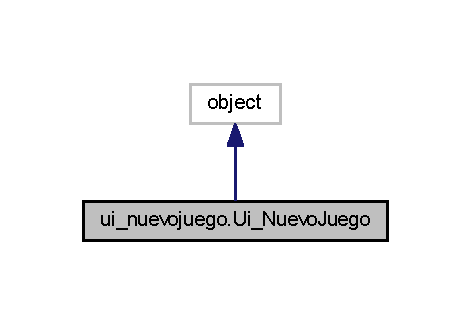
\includegraphics[width=226pt]{classui__nuevojuego_1_1_ui___nuevo_juego__inherit__graph}
\end{center}
\end{figure}


Diagrama de colaboración para ui\-\_\-nuevojuego.\-Ui\-\_\-\-Nuevo\-Juego\-:\nopagebreak
\begin{figure}[H]
\begin{center}
\leavevmode
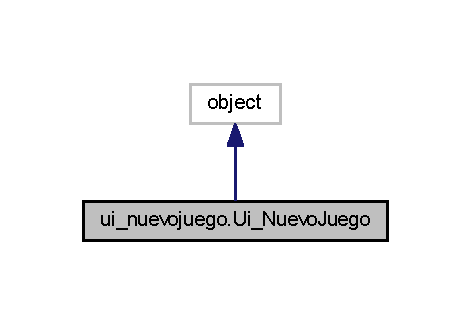
\includegraphics[width=226pt]{classui__nuevojuego_1_1_ui___nuevo_juego__coll__graph}
\end{center}
\end{figure}
\subsection*{Métodos públicos}
\begin{DoxyCompactItemize}
\item 
def {\bfseries setup\-Ui}\label{classui__nuevojuego_1_1_ui___nuevo_juego_ac7a796d972cef2bdb1a9ebeec292d877}

\item 
def {\bfseries retranslate\-Ui}\label{classui__nuevojuego_1_1_ui___nuevo_juego_ad2b5d240f563508e306a321214eb48c0}

\end{DoxyCompactItemize}
\subsection*{Atributos públicos}
\begin{DoxyCompactItemize}
\item 
{\bfseries centralwidget}\label{classui__nuevojuego_1_1_ui___nuevo_juego_a32725a1c9d0ae4f73ea1b0cec5cbdfbe}

\item 
{\bfseries r\-B\-Medio}\label{classui__nuevojuego_1_1_ui___nuevo_juego_a888ccb3b588cbf785b9616702bc3cf39}

\item 
{\bfseries r\-B\-Dificil}\label{classui__nuevojuego_1_1_ui___nuevo_juego_a701cd00892769efdea575c4cb07cec4c}

\item 
{\bfseries r\-B\-Facil}\label{classui__nuevojuego_1_1_ui___nuevo_juego_a60e661f4819967b6d2f09279f49823f4}

\item 
{\bfseries p\-B\-Jugar}\label{classui__nuevojuego_1_1_ui___nuevo_juego_ad4dc95d57abca02628607c7db8595490}

\item 
{\bfseries p\-B\-Cancelar}\label{classui__nuevojuego_1_1_ui___nuevo_juego_a5fe6252995b4373f69fcd50dfa772022}

\item 
{\bfseries r\-B\-Experto}\label{classui__nuevojuego_1_1_ui___nuevo_juego_a4003ba3feb6933eca550eb5ed7523190}

\item 
{\bfseries label}\label{classui__nuevojuego_1_1_ui___nuevo_juego_a7c90438e0dd91760216404e2faf1d3b6}

\item 
{\bfseries label\-\_\-2}\label{classui__nuevojuego_1_1_ui___nuevo_juego_aa983f05d01b60f683dec9796eb59edf2}

\item 
{\bfseries gb\-Op\-Alert}\label{classui__nuevojuego_1_1_ui___nuevo_juego_ac874e4a3457eb4f7edc5c8b24c69afbf}

\item 
{\bfseries cb\-Invalidas}\label{classui__nuevojuego_1_1_ui___nuevo_juego_af2cfdb7c27411d43f24feac3d068e573}

\item 
{\bfseries cb\-Incorrectas}\label{classui__nuevojuego_1_1_ui___nuevo_juego_a4363a573ef6aac3a4d9390d48929101d}

\item 
{\bfseries gb\-Op\-Ayuda}\label{classui__nuevojuego_1_1_ui___nuevo_juego_a0691cb9fb5c75a26a6f74335fc354794}

\item 
{\bfseries cbhelp}\label{classui__nuevojuego_1_1_ui___nuevo_juego_ac2d65ca1dc216e511d8af6b151496516}

\end{DoxyCompactItemize}


La documentación para esta clase fue generada a partir del siguiente fichero\-:\begin{DoxyCompactItemize}
\item 
C\-:/\-Users/\-Kevin/workspace/\-Sudoku\-Python/ui\-\_\-nuevojuego.\-py\end{DoxyCompactItemize}

\section{Referencia de la Clase ui\-\_\-principal.\-Ui\-\_\-principal}
\label{classui__principal_1_1_ui__principal}\index{ui\-\_\-principal.\-Ui\-\_\-principal@{ui\-\_\-principal.\-Ui\-\_\-principal}}


Diagrama de herencias de ui\-\_\-principal.\-Ui\-\_\-principal\nopagebreak
\begin{figure}[H]
\begin{center}
\leavevmode
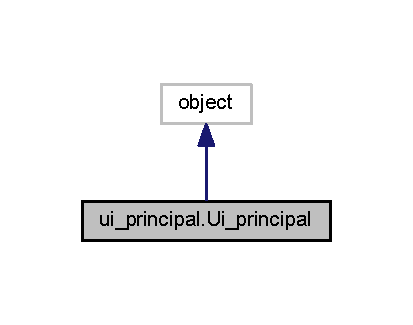
\includegraphics[width=198pt]{classui__principal_1_1_ui__principal__inherit__graph}
\end{center}
\end{figure}


Diagrama de colaboración para ui\-\_\-principal.\-Ui\-\_\-principal\-:\nopagebreak
\begin{figure}[H]
\begin{center}
\leavevmode
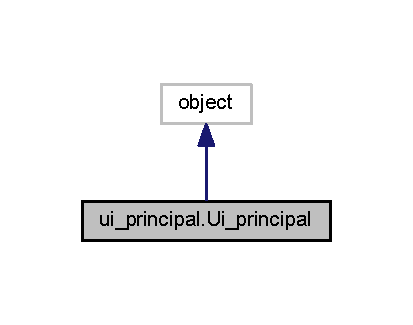
\includegraphics[width=198pt]{classui__principal_1_1_ui__principal__coll__graph}
\end{center}
\end{figure}
\subsection*{Métodos públicos}
\begin{DoxyCompactItemize}
\item 
def {\bfseries setup\-Ui}\label{classui__principal_1_1_ui__principal_ac17bf1466124c2281fdb0f66b93a870c}

\item 
def {\bfseries retranslate\-Ui}\label{classui__principal_1_1_ui__principal_a4890cc7d503f59a780876abc379797f3}

\end{DoxyCompactItemize}
\subsection*{Atributos públicos}
\begin{DoxyCompactItemize}
\item 
{\bfseries centralwidget}\label{classui__principal_1_1_ui__principal_af21a1516c73bfcf451a6bf5fc4267cde}

\item 
{\bfseries icono}\label{classui__principal_1_1_ui__principal_ab41ca5097a5f9d7994c246743c3bd6cb}

\item 
{\bfseries nuevo\-Juego}\label{classui__principal_1_1_ui__principal_ab924923db289b965cb96f702071e066b}

\item 
{\bfseries Carga\-Juego}\label{classui__principal_1_1_ui__principal_a6bc72e32d75a52caafc5ef425eea6559}

\item 
{\bfseries Estadisticas}\label{classui__principal_1_1_ui__principal_aab0480c82cd2d6a0a583781e0501bca0}

\item 
{\bfseries Acerca\-De}\label{classui__principal_1_1_ui__principal_abdea197d8a5851d76ed8108e403ec5b4}

\item 
{\bfseries salir}\label{classui__principal_1_1_ui__principal_a9666b8d6411b41d93fad07e1c610ff79}

\end{DoxyCompactItemize}


La documentación para esta clase fue generada a partir del siguiente fichero\-:\begin{DoxyCompactItemize}
\item 
C\-:/\-Users/\-Kevin/workspace/\-Sudoku\-Python/ui\-\_\-principal.\-py\end{DoxyCompactItemize}

\section{Referencia de la Clase ui\-\_\-sudoku.\-Ui\-\_\-\-Sudoku}
\label{classui__sudoku_1_1_ui___sudoku}\index{ui\-\_\-sudoku.\-Ui\-\_\-\-Sudoku@{ui\-\_\-sudoku.\-Ui\-\_\-\-Sudoku}}


Diagrama de herencias de ui\-\_\-sudoku.\-Ui\-\_\-\-Sudoku\nopagebreak
\begin{figure}[H]
\begin{center}
\leavevmode
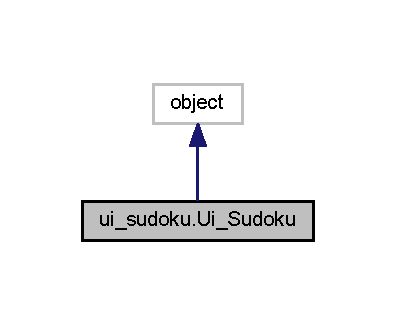
\includegraphics[width=190pt]{classui__sudoku_1_1_ui___sudoku__inherit__graph}
\end{center}
\end{figure}


Diagrama de colaboración para ui\-\_\-sudoku.\-Ui\-\_\-\-Sudoku\-:\nopagebreak
\begin{figure}[H]
\begin{center}
\leavevmode
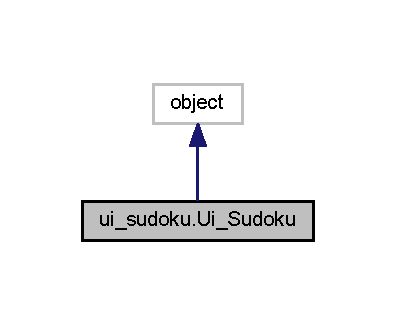
\includegraphics[width=190pt]{classui__sudoku_1_1_ui___sudoku__coll__graph}
\end{center}
\end{figure}
\subsection*{Métodos públicos}
\begin{DoxyCompactItemize}
\item 
def {\bfseries setup\-Ui}\label{classui__sudoku_1_1_ui___sudoku_a975558d747bd8f057dc8361dbee4f6a8}

\item 
def {\bfseries retranslate\-Ui}\label{classui__sudoku_1_1_ui___sudoku_a018e851ec57f840bb31da96699917a19}

\end{DoxyCompactItemize}
\subsection*{Atributos públicos}
\begin{DoxyCompactItemize}
\item 
{\bfseries central\-Widget}\label{classui__sudoku_1_1_ui___sudoku_a2301cee8d2de21fad31bac7d9929c501}

\item 
{\bfseries horizontal\-Layout}\label{classui__sudoku_1_1_ui___sudoku_ad15cdd7e6072c1f49ce54899a1c458ad}

\item 
{\bfseries g\-L\-Tablero}\label{classui__sudoku_1_1_ui___sudoku_ad66ebdce406d7a9a601a84a451bf638e}

\item 
{\bfseries grid\-Layout}\label{classui__sudoku_1_1_ui___sudoku_acfc8f17199ae55d62d336bf60e412625}

\item 
{\bfseries gl\-Pistas}\label{classui__sudoku_1_1_ui___sudoku_a5ee37a30e3a8ca9f49d7695ea09ea9e5}

\item 
{\bfseries p\-Bf3}\label{classui__sudoku_1_1_ui___sudoku_adddd39056c8a6cfe3301101842b6f266}

\item 
{\bfseries p\-Bf4}\label{classui__sudoku_1_1_ui___sudoku_acf867d79729618c2a213d62da489bc3c}

\item 
{\bfseries cont\-Tiempo}\label{classui__sudoku_1_1_ui___sudoku_ac406346f8929bc2091a6c663a5852984}

\item 
{\bfseries p\-Bf1}\label{classui__sudoku_1_1_ui___sudoku_a00af531da13f6987b806b5ed4e1084fc}

\item 
{\bfseries p\-Bf2}\label{classui__sudoku_1_1_ui___sudoku_a844c80d75a61e67673665675ddb6b38e}

\item 
{\bfseries p\-Bf5}\label{classui__sudoku_1_1_ui___sudoku_a409facddb839cfce9cae3a25c51dd119}

\item 
{\bfseries p\-Bf6}\label{classui__sudoku_1_1_ui___sudoku_a69dfec0542034ea467e5108f8ecd984e}

\item 
{\bfseries p\-Bf7}\label{classui__sudoku_1_1_ui___sudoku_a251bebee338297e5d2988eb9d978d1a3}

\item 
{\bfseries p\-Bf8}\label{classui__sudoku_1_1_ui___sudoku_afe9cddecea36350c214cfc15a21b4c96}

\item 
{\bfseries p\-Bf9}\label{classui__sudoku_1_1_ui___sudoku_a9619bb01455b1f53d8c608b538d2c079}

\item 
{\bfseries bt\-Help}\label{classui__sudoku_1_1_ui___sudoku_a81b9e3c1660226443fa6bec0bee23757}

\item 
{\bfseries label\-\_\-3}\label{classui__sudoku_1_1_ui___sudoku_abca320418644674c78c90113caa9d007}

\item 
{\bfseries label}\label{classui__sudoku_1_1_ui___sudoku_a5ff3ec94e5146b1e44d91cc6c6cff0df}

\item 
{\bfseries label\-\_\-2}\label{classui__sudoku_1_1_ui___sudoku_a09be504022ccbdf442f44d9216f4c4f0}

\item 
{\bfseries label\-\_\-4}\label{classui__sudoku_1_1_ui___sudoku_afeca417cad8816ec1d71d9f1a8e98d8b}

\item 
{\bfseries menu\-Bar}\label{classui__sudoku_1_1_ui___sudoku_abbddb844a0b7c26a8a04d2ee23afe483}

\item 
{\bfseries menu\-Archivo}\label{classui__sudoku_1_1_ui___sudoku_a1fbe1c494eb2ce64065f0ae57aad1945}

\item 
{\bfseries action\-Nuevo\-\_\-\-Juego}\label{classui__sudoku_1_1_ui___sudoku_af204cd509001d0f55ee9dafbe94d458d}

\item 
{\bfseries action\-Salir}\label{classui__sudoku_1_1_ui___sudoku_a9115deb8db150443670a16146c6b4c49}

\item 
{\bfseries action\-Mostrar\-\_\-\-Solucion}\label{classui__sudoku_1_1_ui___sudoku_a5bcdb6d83bf7f25b8f3340194595322f}

\item 
{\bfseries action\-Guardar}\label{classui__sudoku_1_1_ui___sudoku_a4c7efdf64560c6a4e4fa22da0abeed97}

\end{DoxyCompactItemize}


La documentación para esta clase fue generada a partir del siguiente fichero\-:\begin{DoxyCompactItemize}
\item 
C\-:/\-Users/\-Kevin/workspace/\-Sudoku\-Python/ui\-\_\-sudoku.\-py\end{DoxyCompactItemize}

\section{Referencia de la Clase validador.\-Validador}
\label{classvalidador_1_1_validador}\index{validador.\-Validador@{validador.\-Validador}}


Clase que maneja las validaciones del numero dentro del tablero.  


\subsection*{Métodos públicos}
\begin{DoxyCompactItemize}
\item 
def {\bf \-\_\-\-\_\-init\-\_\-\-\_\-}
\item 
def {\bf Relacionar}
\item 
def {\bf Validar\-Espacios\-Vacios}
\item 
def {\bf Sub\-Cuadros}
\item 
def {\bf Verificar\-Sub\-Cuadro}
\item 
def {\bf Validar\-X}
\item 
def {\bf Valida\-Linea}
\item 
def {\bf Validar\-Y}
\item 
def {\bf Valida\-Columna}
\item 
def {\bf Verifica\-Arreglo\-Indices}
\item 
def {\bf Validaciones}
\end{DoxyCompactItemize}
\subsection*{Atributos públicos}
\begin{DoxyCompactItemize}
\item 
{\bfseries sudoku}\label{classvalidador_1_1_validador_ab02c154c37d3454eb353a95a5aed20f8}

\item 
{\bfseries graficador}\label{classvalidador_1_1_validador_a526c2702b5b2c184889627da16f01df9}

\item 
{\bfseries Message\-Box}\label{classvalidador_1_1_validador_ad586789a4610f21e37909feea08fb221}

\item 
{\bfseries M\-B\-\_\-\-I\-C\-O\-N\-E\-R\-R\-O\-R}\label{classvalidador_1_1_validador_ac14bb6e1aeac4173c44a0596b611d3fd}

\end{DoxyCompactItemize}


\subsection{Descripción detallada}
Clase que maneja las validaciones del numero dentro del tablero. 



\subsection{Documentación del constructor y destructor}
\index{validador\-::\-Validador@{validador\-::\-Validador}!\-\_\-\-\_\-init\-\_\-\-\_\-@{\-\_\-\-\_\-init\-\_\-\-\_\-}}
\index{\-\_\-\-\_\-init\-\_\-\-\_\-@{\-\_\-\-\_\-init\-\_\-\-\_\-}!validador::Validador@{validador\-::\-Validador}}
\subsubsection[{\-\_\-\-\_\-init\-\_\-\-\_\-}]{\setlength{\rightskip}{0pt plus 5cm}def validador.\-Validador.\-\_\-\-\_\-init\-\_\-\-\_\- (
\begin{DoxyParamCaption}
\item[{}]{self, }
\item[{}]{Sudoku}
\end{DoxyParamCaption}
)}\label{classvalidador_1_1_validador_a7504d5eaa60d9a8410ab9dcdf6e906f1}
\begin{DoxyVerb}Contructor
    Se Inicializa la variable del tablero para tener acceso a este y creamos un objeto de tipo graficador para poder pintar el tablero.
    Parametro:
    s El objeto padre de tipo Sudoku que crea a este objeto.\end{DoxyVerb}
 

\subsection{Documentación de las funciones miembro}
\index{validador\-::\-Validador@{validador\-::\-Validador}!Relacionar@{Relacionar}}
\index{Relacionar@{Relacionar}!validador::Validador@{validador\-::\-Validador}}
\subsubsection[{Relacionar}]{\setlength{\rightskip}{0pt plus 5cm}def validador.\-Validador.\-Relacionar (
\begin{DoxyParamCaption}
\item[{}]{self}
\end{DoxyParamCaption}
)}\label{classvalidador_1_1_validador_ae52c0b87f72d4d23b31d63a383eed6f3}
\begin{DoxyVerb}Pasa de la imagen de la ficha a un entero que corresponde al numero de la imagen.\end{DoxyVerb}
 \index{validador\-::\-Validador@{validador\-::\-Validador}!Sub\-Cuadros@{Sub\-Cuadros}}
\index{Sub\-Cuadros@{Sub\-Cuadros}!validador::Validador@{validador\-::\-Validador}}
\subsubsection[{Sub\-Cuadros}]{\setlength{\rightskip}{0pt plus 5cm}def validador.\-Validador.\-Sub\-Cuadros (
\begin{DoxyParamCaption}
\item[{}]{self}
\end{DoxyParamCaption}
)}\label{classvalidador_1_1_validador_a6a696985f736a08f0c4e68f4c41a696d}
\begin{DoxyVerb}Extrae la subcuadricula en la que se va a buscar algun posible numero repetido.
    Retorna: 1 -> Correcto , 0 -> Existen numeros repetidos\end{DoxyVerb}
 \index{validador\-::\-Validador@{validador\-::\-Validador}!Validaciones@{Validaciones}}
\index{Validaciones@{Validaciones}!validador::Validador@{validador\-::\-Validador}}
\subsubsection[{Validaciones}]{\setlength{\rightskip}{0pt plus 5cm}def validador.\-Validador.\-Validaciones (
\begin{DoxyParamCaption}
\item[{}]{self}
\end{DoxyParamCaption}
)}\label{classvalidador_1_1_validador_a38428f3a8424457f6d1fac000c22b826}
\begin{DoxyVerb}Maneja todas las validaciones y muestra un mensaje al usuario de acuerdo al tipo de error.
    Retorna: 1 -> Correcto , 0 -> Existen numeros repetidos.\end{DoxyVerb}
 \index{validador\-::\-Validador@{validador\-::\-Validador}!Valida\-Columna@{Valida\-Columna}}
\index{Valida\-Columna@{Valida\-Columna}!validador::Validador@{validador\-::\-Validador}}
\subsubsection[{Valida\-Columna}]{\setlength{\rightskip}{0pt plus 5cm}def validador.\-Validador.\-Valida\-Columna (
\begin{DoxyParamCaption}
\item[{}]{self, }
\item[{}]{j}
\end{DoxyParamCaption}
)}\label{classvalidador_1_1_validador_a181d6a109b73f81c7addfd28f4422855}
\begin{DoxyVerb}Busca en la columna j si existe algun numero repetido.
    Parametro: j Columna donde se buscara.
    Retorna: Valor: 1 -> Correcto , 0 -> Existen numeros repetidos.\end{DoxyVerb}
 \index{validador\-::\-Validador@{validador\-::\-Validador}!Valida\-Linea@{Valida\-Linea}}
\index{Valida\-Linea@{Valida\-Linea}!validador::Validador@{validador\-::\-Validador}}
\subsubsection[{Valida\-Linea}]{\setlength{\rightskip}{0pt plus 5cm}def validador.\-Validador.\-Valida\-Linea (
\begin{DoxyParamCaption}
\item[{}]{self, }
\item[{}]{i}
\end{DoxyParamCaption}
)}\label{classvalidador_1_1_validador_a2e9acd907c83b25cb509598535b89199}
\begin{DoxyVerb}Busca en la linea i si existe algun numero repetido.
    Parametro: i Linea donde se buscara.
    Retorna: 1 -> Correcto , 0 -> Existen numeros repetidos.\end{DoxyVerb}
 \index{validador\-::\-Validador@{validador\-::\-Validador}!Validar\-Espacios\-Vacios@{Validar\-Espacios\-Vacios}}
\index{Validar\-Espacios\-Vacios@{Validar\-Espacios\-Vacios}!validador::Validador@{validador\-::\-Validador}}
\subsubsection[{Validar\-Espacios\-Vacios}]{\setlength{\rightskip}{0pt plus 5cm}def validador.\-Validador.\-Validar\-Espacios\-Vacios (
\begin{DoxyParamCaption}
\item[{}]{self}
\end{DoxyParamCaption}
)}\label{classvalidador_1_1_validador_aa24ab8d3da4ac839f41cf4615637e2b2}
\begin{DoxyVerb}Verifica si el en tablero hay algun espacio vacio
    Retorna: 1 -> Completo , 0 -> Incompleto.\end{DoxyVerb}
 \index{validador\-::\-Validador@{validador\-::\-Validador}!Validar\-X@{Validar\-X}}
\index{Validar\-X@{Validar\-X}!validador::Validador@{validador\-::\-Validador}}
\subsubsection[{Validar\-X}]{\setlength{\rightskip}{0pt plus 5cm}def validador.\-Validador.\-Validar\-X (
\begin{DoxyParamCaption}
\item[{}]{self}
\end{DoxyParamCaption}
)}\label{classvalidador_1_1_validador_aaf155f90206e777346f6fc4b81a19880}
\begin{DoxyVerb}Recorre el tablero linea a linea para encontrar numeros repetidos
Retorna: 1 -> Correcto , 0 -> Existen numeros repetidos.\end{DoxyVerb}
 \index{validador\-::\-Validador@{validador\-::\-Validador}!Validar\-Y@{Validar\-Y}}
\index{Validar\-Y@{Validar\-Y}!validador::Validador@{validador\-::\-Validador}}
\subsubsection[{Validar\-Y}]{\setlength{\rightskip}{0pt plus 5cm}def validador.\-Validador.\-Validar\-Y (
\begin{DoxyParamCaption}
\item[{}]{self}
\end{DoxyParamCaption}
)}\label{classvalidador_1_1_validador_a9c91760d11975839c73ccaf9586c9772}
\begin{DoxyVerb}Recorre el tablero columna a columna para encontrar numeros repetidos
    Retorna: 1 -> Correcto , 0 -> Existen numeros repetidos.\end{DoxyVerb}
 \index{validador\-::\-Validador@{validador\-::\-Validador}!Verifica\-Arreglo\-Indices@{Verifica\-Arreglo\-Indices}}
\index{Verifica\-Arreglo\-Indices@{Verifica\-Arreglo\-Indices}!validador::Validador@{validador\-::\-Validador}}
\subsubsection[{Verifica\-Arreglo\-Indices}]{\setlength{\rightskip}{0pt plus 5cm}def validador.\-Validador.\-Verifica\-Arreglo\-Indices (
\begin{DoxyParamCaption}
\item[{}]{self, }
\item[{}]{fichas}
\end{DoxyParamCaption}
)}\label{classvalidador_1_1_validador_a25eea8cc26b574744fc794cd0d8f9c4a}
\begin{DoxyVerb}Verifica el numero de veces que se repite un numero.
    Si algun numero se repite mas de una vez, entonces existe algun repetido.
    Parametro: fichas Numero de ocurrencias de cada numero.
    Retorna: 1 -> Correcto , 0 -> Existen numeros repetidos.\end{DoxyVerb}
 \index{validador\-::\-Validador@{validador\-::\-Validador}!Verificar\-Sub\-Cuadro@{Verificar\-Sub\-Cuadro}}
\index{Verificar\-Sub\-Cuadro@{Verificar\-Sub\-Cuadro}!validador::Validador@{validador\-::\-Validador}}
\subsubsection[{Verificar\-Sub\-Cuadro}]{\setlength{\rightskip}{0pt plus 5cm}def validador.\-Validador.\-Verificar\-Sub\-Cuadro (
\begin{DoxyParamCaption}
\item[{}]{self}
\end{DoxyParamCaption}
)}\label{classvalidador_1_1_validador_a64dc72d82bd892b5330d0584bc244cfb}
\begin{DoxyVerb}Valida que no existan numeros repetidos en la subcuadricula.
    En caso de haber algun numero repetido en la subcuadricula, se pinta dicha subcuadricula.
    Retorna: 1 -> Correcto , 0 -> Existen numeros repetidos\end{DoxyVerb}
 

La documentación para esta clase fue generada a partir del siguiente fichero\-:\begin{DoxyCompactItemize}
\item 
C\-:/\-Users/\-Kevin/workspace/\-Sudoku\-Python/validador.\-py\end{DoxyCompactItemize}

%--- End generated contents ---

% Index
\newpage
\phantomsection
\addcontentsline{toc}{part}{Índice}
\printindex

\end{document}
